\newpage
\appendix
\onecolumn

\section{Proof}
\label{appsec:proof}
In this section, we provide proofs for the theorems presented in the main paper.
\subsection{Proof of Theorem \ref{thm:quantize_error}}
\label{proof:quantize_error}

\begin{theorem}[Restated, \ref{thm:quantize_error}]
Let \( \mathbf{x} \in \mathbb{R}^d \) be a vector, and let the quantization bandwidth be \( b \in \mathbb{N} \). Define the max-min dynamic quantizer as follows:
\begin{gather}
\label{eqn:s}
    s  = \frac{\max(\mathbf{x}) - \min(\mathbf{x})}{2^b - 1}, \\
    \mathbf{z}  = \left\lfloor -\frac{\min(\mathbf{x})}{s} \right\rfloor, \\
    \mathbf{x}_\text{int}  = \text{clamp}(\left\lfloor \frac{\mathbf{x}}{s} \right\rfloor + \mathbf{z}, 0, 2^b-1).
\end{gather}
The corresponding dequantization is given by:
\begin{equation}
    Q(\mathbf{x}) = s (\mathbf{x}_\text{int} - \mathbf{z}).
\end{equation}

The quantization error is bounded in terms of the quantization scaling factor \( s \), which depends on the range of \( \mathbf{x} \) and the bandwidth \( b \). Specifically, we have:
\begin{equation}
    \|\mathbf{x} - Q(\mathbf{x})\|_2^2 \leq {s^2d} = \frac{(\max(\mathbf{x}) - \min(\mathbf{x}))^2d}{(2^b - 1)^2}.
\end{equation}
\end{theorem}


\textit{Proof:} For any \( i \in \{1, 2, \dots, d\} \), the value \( x_i \) satisfies the following property:

\begin{align}
    0 \leq \lfloor \frac{\min(\vx)}{s} \rfloor + \lfloor \frac{-\min(\vx)}{s} \rfloor 
    \leq \lfloor \frac{x_i}{s} \rfloor + z 
    \leq \lfloor \frac{\max(\vx)}{s} \rfloor + \lfloor \frac{-\min(\vx)}{s} \rfloor 
    \leq \frac{\max(\vx) - \min(\vx)}{s}.
\end{align}

From condition (~\ref{eqn:s}), we have:
\[
0 \leq x_{\text{int}} \leq 2^b - 1.
\]
This ensures that the clipping error is zero, meaning we only need to consider the rounding error. Thus, we obtain:
\begin{align}
    x_i - Q(x)_i &= x_i - \lfloor \frac{x_i}{s} \rfloor s \\
    &= s \left( \frac{x_i}{s} - \lfloor \frac{x_i}{s} \rfloor \right) \leq s.
\end{align}

Therefore, applying this to the \( \ell_2 \)-norm error bound, we derive:
\begin{align}
    \| \vx - Q(\vx) \|_2^2 
    &= \sum_{i=1}^{d} (x_i - Q(x)_i)^2 \\
    &\leq \sum_{i=1}^{d} s^2 \\
    &= s^2 d.
\end{align}
\hfill\(\square\)


\subsection{Proof of Theorem \ref{thm:acc_error}}
\label{proof:acc_error}
\begin{theorem}[Restated, \ref{thm:acc_error}]
Let \(\mathcal{A}(\cdot)\) be a linear operator and consider a sequence of inputs \(\mathbf{a}_T, \mathbf{a}_{T-1}, \dots, \mathbf{a}_1\), with corresponding outputs \(\mathbf{o}_T, \mathbf{o}_{T-1}, \dots, \mathbf{o}_1\). Given a quantization operator \(Q\), we estimate the outputs using standard modulation: 
\begin{align}
\label{eqn:modulation}
    \tilde{\mathbf{o}}_t &= \mathcal{A}(Q(\mathbf{a}_t - \mathbf{a}_{t+1})) + \tilde{\mathbf{o}}_{t+1}, \\
\label{eqn:ecmodulation}
    \tilde{\mathbf{o}}_T &= \mathcal{A}(\mathbf{a}_T),
\end{align}
where \( t = T-1, \dots, 2, 1 \). Similarly, we estimate the outputs using error-compensated modulation:  
\begin{align}
    \hat{\mathbf{o}}_t &= \mathcal{A}(Q(\mathbf{a}_t - \hat{\mathbf{a}}_{t+1})) + \hat{\mathbf{o}}_{t+1}, \\
    \hat{\mathbf{a}}_t &= Q(\mathbf{a}_t - \hat{\mathbf{a}}_{t+1}) + \hat{\mathbf{a}}_{t+1}, \\
    \hat{\mathbf{o}}_T &= \mathcal{A}(\mathbf{a}_T), \quad
    \hat\va_T = \va_T,
\end{align}
where \( t = T-1, \dots, 2, 1 \). Suppose the quantization operator \(Q\) satisfies the following error bound: 
\begin{align}
    \|\mathbf{x} - Q(\mathbf{x})\|_2^2 \leq c\|\mathbf{x}\|_2^2, \quad 0 < c < \frac{1}{2}.
\end{align}
Then, the estimation errors are bounded as follows:  
\begin{align}
\label{eqn:con1}
    \|\mathbf{o}_t - \tilde{\mathbf{o}}_t\|_2^2 &\leq \sum_{k=t}^{T-1} 2^{T-k-1} c \|\mathcal{A}\|_2^2 \|\mathbf{a}_k - \mathbf{a}_{k+1}\|_2^2, \\
    \label{eqn:con2}
    \|\mathbf{o}_t - \hat{\mathbf{o}}_t\|_2^2 &\leq \sum_{k=t}^{T-1} (2c)^{T-k-1} \|\mathcal{A}\|_2^2 \|\mathbf{a}_k - \mathbf{a}_{k+1}\|_2^2.
\end{align}
\end{theorem}

\textit{Proof:} Denote the error for standard modulation in Equation (\ref{eqn:modulation}) as $\tilde\ve_t$ and for error-compensation modulation in Equation (\ref{eqn:ecmodulation}) as $\hat\ve_t$ at time step $t$. We first compute the error for standard modulation:
\begin{align}
    \tilde\ve_t^2 &= \|\vo_t-\tilde\vo_t\|_2^2 \\
    &= \|\vo_t-\cA(Q(\va_t-\va_{t+1}))-\tilde\vo_{t+1}\|_2^2 \\
    &= \|\vo_t-\vo_{t+1}-\cA(Q(\va_t-\va_{t+1}))+(\vo_{t+1}-\tilde\vo_{t+1})\|_2^2 \\
    &= \|\cA(\va_t-\va_{t+1})-\cA(Q(\va_t-\va_{t+1}))+(\vo_{t+1}-\tilde\vo_{t+1})\|_2^2 \\
    &= \|\cA(\va_t-\va_{t+1}-Q(\va_t-\va_{t+1}))+(\vo_{t+1}-\tilde\vo_{t+1})\|_2^2 \\
    &\leq 2|\cA(\va_t-\va_{t+1}-Q(\va_t-\va_{t+1}))\|_2^2 + 2\|\vo_{t+1}-\tilde\vo_{t+1}\|_2^2 
\end{align}
Since $\|(\vo_{t+1}-\tilde\vo_{t+1})\|_2^2$ represents the error from the previous time step, applying the submultiplicative inequality yields:
\begin{align}
    \tilde\ve_t^2 &= \|\vo_t-\tilde\vo_t\|_2^2 \\
    & \leq 2\|\cA\|_2^2\|\va_t-\va_{t+1}-Q(\va_t-\va_{t+1})\|_2^2 + 2\ve_{t+1}^2 \\
    & \leq 2c\|\cA\|_2^2\|\va_t-\va_{t+1}\|_2^2 + 2\ve_{t+1}^2, 
\end{align}
Accumulating the error from time $T$ to $t$, we obtain Equation (\ref{eqn:con1}).

For the error-compensation modulation, we compute:
\begin{align}
    \hat\ve_t^2 &= \|\vo_t-\hat\vo_t\|_2^2 \\
    &= \|\vo_t-\cA(Q(\va_t-\hat\va_{t+1}))-\hat\vo_{t+1}\|_2^2 \\
    & = \|\cA(\va_t)-\cA(Q(\va_t-\hat\va_{t+1}))-\cA(\hat\va_{t+1})\|_2^2 \\
    & =\|\cA(\va_t-\hat\va_{t+1}-Q(\va_t-\hat\va_{t+1}))\|_2^2 \\
    \label{eqn:65}
    &\leq c\|\cA\|_2^2\|\va_t-\hat\va_{t+1}\|_2^2
\end{align}
Next, we expand $\va_t-\hat\va_{t+1}$:
\begin{align}
    \|\va_t-\hat\va_{t+1}\|_2^2 &= \|\va_t-Q(\va_{t+1}-\hat\va_{t+2})-\hat\va_{t+2}\|_2^2 \\
    & = \|\va_t-\va_{t+1}-Q(\va_{t+1}-\hat\va_{t+2})+\va_{t+1}-\hat\va_{t+2}\|_2^2 \\
    & \leq 2\|\va_t-\va_{t+1}\|_2^2+2\|Q(\va_{t+1}-\hat\va_{t+2})+\va_{t+1}-\hat\va_{t+2}\|_2^2 \\
    & \leq 2\|\va_t-\va_{t+1}\|_2^2+2c\|\va_{t+1}-\hat\va_{t+2}\|_2^2
\end{align}
Substituting this into Equation (\ref{eqn:65}), we complete the proof. 
\hfill$\square$

\subsection{Proof of Corollary}
\label{subsec:corollary}
\begin{corollary}
Let \( \mathbf{x} \in \mathbb{R}^d \) be a vector, and let the quantization bandwidth be \( b \in \mathbb{N} \). Define the max-min dynamic quantizer as follows:
\begin{gather}
    s  = \frac{\max(\mathbf{x}) - \min(\mathbf{x})}{2^b - 1}, \\
    \mathbf{z}  = \left\lfloor -\frac{\min(\mathbf{x})}{s} \right\rfloor, \\
    \mathbf{x}_\text{int}  = \text{clamp}(\left\lfloor \frac{\mathbf{x}}{s} \right\rfloor + \mathbf{z}, 0, 2^b-1).
\end{gather}
The corresponding dequantization is given by:
\begin{equation}
    Q(\mathbf{x}) = s (\mathbf{x}_\text{int} - \mathbf{z}).
\end{equation}
For any $0<c<\frac{1}{2}$, we can revise $Q$ with a new bandwidth $\hat b$ satisfying:
\begin{align}
    \|\vx- Q(\vx)\|_2^2\leq c\|\vx\|_2^2.
\end{align}
\end{corollary}

\textit{Proof:} From Theorem~\ref{thm:quantize_error}, we have:
\begin{align}
    \|\mathbf{x} - Q(\mathbf{x})\|_2^2 &\leq \frac{(\max(\mathbf{x}) - \min(\mathbf{x}))^2d}{(2^b - 1)^2} \\
    & \leq \frac{4\|\vx\|_\infty^2d}{(2^b - 1)^2} \\
    & \leq \frac{4\|\vx\|_2^2d}{(2^b - 1)^2}
\end{align}
To satisfy the desired bound, we choose $\hat{b}$ such that: \begin{align} \hat{b} \geq \log_2\left(\sqrt{\frac{4d}{c}} + 1\right). \end{align} Thus, the proof is complete. \hfill$\square$

\section{Implementation details}
\label{appsec:implement}
In this section, we talk about the hyperparameters in our experiments and the implementation details of our MoDiff. 

\textbf{Baselines.}
For the implementation of baselines, we follow the existing codebase. Specifically, we conduct Q-Diffusion experiments by directly using their provided code~\citep{li2023q}. We also utilize the calibration datasets they provide to quantize the models at different bit levels. For LCQ, we follow the BRECQ framework and adopt channel-wise quantization~\citep{li2021brecq}.

\textbf{MoDiff.}
For our MoDiff implementation, we incorporate several key techniques: 
\begin{itemize}
\item Bias Removal: We remove all bias terms from layers that apply MoDiff. This is necessary because our method, as described in Equation (\ref{ec5}), requires layers to be bias-free to prevent unwanted accumulation of bias terms.

\item Warm-up: We apply warm-up at the first step, where we use full activation for computation. More detailed analysis is shown in Appendix~\ref{appsec:warmup}.

\item Calibration Dataset Reconstruction: We reconstruct the calibration dataset for Q-Diff + MoDiff, ensuring it captures nearby information. During calibration, we store the inputs and outputs of MoDiff rather than the raw activations.

\item Layer-wise Reconstruction: Instead of reconstructing entire blocks, we reconstruct each layer individually, as we find this approach leads to more stable performance.

\item Hyperparameter Consistency: We do not fine-tune the calibration hyperparameters, as optimizing them is not the primary focus of our work.

\end{itemize}

\section{Additional Main Results}

\subsection{Results on Stable Diffusion}
\label{appse: stable}

To demonstrate that our method generalizes to larger-scale datasets and higher resolutions, we conduct experiments on MS-COCO 2014~\citep{lin2014microsoft} using Stable Diffusion v1.4 with DPM solvers\citep{lu2022dpm}. We apply tensor-wise dynamic quantization and evaluate the quantized models within the Q-Diffusion framework. A total of 30,000 images are generated using 50 sampling steps. As shown in Table~\ref{tab:stable}, the resulting FID scores confirm that MoDiff consistently performs well on large-scale diffusion models.

\begin{table}[h!]
\centering
\caption{The FID and sFID on MS-COCO with Stable Diffusion using PLMS solver under different precisions. The best performance is \textbf{bolded}.}
\begin{tabular}{l|c|c|c}
\toprule
{Methods} & {Bits (W/A)} & FID $\downarrow$ & sFID $\downarrow$ \\
\midrule
LTQ & \multirow{2}{*}{8/8} & 12.15 & 19.05 \\
LTQ+MoDiff (Ours) & & \bf 12.14 & \bf 19.05 \\
\midrule
LTQ & \multirow{2}{*}{8/6} & 71.38 & 59.74 \\
LTQ+MoDiff (Ours) & & \bf 13.21 & \bf 20.07 \\
\midrule
LTQ & \multirow{2}{*}{8/4} & 408.42 & 199.59 \\
LTQ+MoDiff (Ours) & & \bf 225.22 & \bf 104.12 \\
\bottomrule
\end{tabular}
\label{tab:stable}
\end{table}

\subsection{Results on Transformer-Based Models}
\label{appsec: DiT}
To evaluate the generalizability of MoDiff across different architectures, we conduct experiments on the Diffusion Transformer~\citep{peebles2023scalable}. Following PTQ4DiT~\citep{wu2024ptq4dit}, we use DiT-XL/2 as the baseline model. The experiments are performed on the ImageNet 256×256 dataset~\citep{ILSVRC15} using tensor-wise dynamic quantization. We generate 10,000 images using 50 sampling steps for evaluation. As shown in Table~\ref{tab:DiT}, MoDiff consistently enhances generation quality under low activation bit widths.

\begin{table}[h!]
\centering
\caption{The IS, FID, and sFID for ImageNet 256x256 with DiT-XL/2 under different precisions. The best performance is \textbf{bolded}.}
\begin{tabular}{l|c|c|c|c}
\toprule
{Methods} & {Bits (W/A)} & IS $\uparrow$ & FID $\downarrow$ & sFID $\downarrow$ \\
\midrule
PTQ4DiT & \multirow{2}{*}{8/8} & 36.91 & 54.80 & 89.60 \\
PTQ4DiT+MoDiff (Ours) & & \bf 37.37 & \bf 53.76 & \bf 89.53 \\
\midrule
PTQ4DiT & \multirow{2}{*}{8/6} & 3.41 & 200.26 & 373.71 \\
PTQ4DiT+MoDiff (Ours) & & \bf 36.74 & \bf 54.74 & \bf 88.49 \\
\midrule
PTQ4DiT & \multirow{2}{*}{8/4} & 1.45 & 271.87 & 207.59 \\
PTQ4DiT+MoDiff (Ours) & & \bf 17.23 & \bf 90.91 & \bf 102.07 \\
\bottomrule
\end{tabular}
\label{tab:DiT}
\end{table}


\subsection{More Measurements on Generation Quality}
In the main paper, we evaluate the quality of generated outputs using Inception Score (IS), Fréchet Inception Distance (FID), and sFID. Here, we further assess the performance of our method using precision and recall. 

The results are presented in Table~\ref{tab:cifar10_pr}, Table~\ref{tab:church_pr}, and Table~\ref{tab:bedroom_pr}. These results demonstrate that MoDiff effectively preserves precision and recall even at low activation bit levels. For instance, on CIFAR-10, LCQ+MoDiff achieves a precision of 0.58 and a recall of 0.50, whereas LCQ alone results in 0 for both metrics.

\label{appsec:measurements}
\begin{table*}[!ht]
\small
\centering
\caption{The Precision and Recall for CIFAR-10 with DDIM under different Bits. The best performance is \textbf{bolded}.}
\begin{tabular}{l|c|cc||c|ccc}
\toprule
{Methods} & {Bits (W/A)} & Precision & Recall & {Bits (W/A)} & Precision  & Recall & \\
\midrule
Full Prec. (Act) & 8/32 & 0.65 & 0.55 & 4/32 & 0.64 & 0.56\\
\midrule
Q-Diff & \multirow{4}{*}{8/8} & 0.65 & 0.55 & \multirow{4}{*}{4/8} & 0.66 & 0.58 \\
Q-Diff+MoDiff (Ours) & & 0.65 & 0.56 & & 0.65 & 0.58 & \\
LCQ & & 0.67 & 0.59 & & 0.67 & 0.57 & \\
LCQ+MoDiff (Ours) & & 0.66 & 0.59 & & 0.67 & 0.55 & \\
\midrule
Q-Diff & \multirow{4}{*}{8/6} & 0.46 & 0.47 & \multirow{4}{*}{4/6} & 0.47 & 0.44 \\
Q-Diff+MoDiff (Ours) & & 0.66 & 0.57 & & 0.65 & 0.59 & \\
LCQ & & 0.67 & 0.58 & & 0.67 & 0.57 & \\
LCQ+MoDiff (Ours) & & 0.66 & 0.58 & & 0.67 & 0.56 & \\
\midrule
Q-Diff & \multirow{4}{*}{8/4} & 0.08 & 0.00 & \multirow{4}{*}{4/4} & 0.05 & 0.00 \\
Q-Diff+MoDifff(Ours) & & 0.54 & 0.53 & & 0.53 & 0.55 & \\
LCQ & & 0.47 & 0.44 & & 0.48 & 0.43 & \\
LCQ+MoDiff (Ours) & & 0.67 & 0.59 & & 0.67 & 0.57 & \\
\midrule
Q-Diff & \multirow{4}{*}{8/3} & 0.00 & 0.00 & \multirow{4}{*}{4/3} & 0.00 & 0.00 \\
Q-Diff+MoDiff (Ours) & & 0.45 & 0.39 & & 0.33 & 0.32 & \\
LCQ & & 0.33 & 0.08 & & 0.35 & 0.08 & \\
LCQ+MoDiff (Ours)& & 0.66 & 0.59 & & 0.67 & 0.57 & \\
\midrule
Q-Diff & \multirow{4}{*}{8/2} & 0.00 & 0.00 & \multirow{4}{*}{4/2} & 0.00 & 0.00 \\
Q-Diff+MoDiff (Ours) & & 0.00 & 0.00 & & 0.14 & 0.00 & \\
LCQ & & 0.00 & 0.00 & & 0.00 & 0.00 & \\
LCQ+MoDiff (Ours) & & 0.58 & 0.50 & & 0.58 & 0.47 & \\
\bottomrule
\end{tabular}
\label{tab:cifar10_pr}
\end{table*}


\begin{table*}[!ht]
\small
\centering
\caption{The Precision and Recall for Church with LDM-8 under different Bits. The best performance is \textbf{bolded}.}
\begin{tabular}{l|c|cc||c|ccc}
\toprule
{Methods} & {Bits (W/A)} & Precision & Recall & {Bits (W/A)} & Precision  & Recall & \\
\midrule
Full Prec. (Act) & 8/32 & 0.63 & 0.51 & 4/32 & 0.63 & 0.52 \\
\midrule
LCQ & \multirow{2}{*}{8/8} & 0.62 & 0.47 & \multirow{2}{*}{4/8} & 0.62 & 0.46 & \\
LCQ+MoDiff (Ours) & & 0.63 & 0.53 & & 0.63 & 0.53 & \\
\midrule
LCQ & \multirow{2}{*}{8/6}& 0.59 & 0.46 & \multirow{2}{*}{4/6}& 0.59 & 0.45 & \\
LCQ+MoDiff (Ours) & & 0.63 & 0.53 & & 0.63 & 0.53 & \\
\midrule
LCQ & \multirow{2}{*}{8/4}& 0.03 & 0.14 & \multirow{2}{*}{4/4}& 0.02 & 0.07 & \\
LCQ+MoDiff (Ours) & & 0.63 & 0.53 & & 0.63 & 0.5 & \\
\midrule
LCQ &\multirow{2}{*}{8/3} & 0.00 & 0.00 &\multirow{2}{*}{4/3} & 0.00 & 0.00 & \\
LCQ+MoDiff (Ours)& & 0.61 & 0.34 & & 0.60 & 0.34 & \\
\bottomrule
\end{tabular}
\label{tab:church_pr}
\end{table*}


\begin{table*}[!ht]
\small
\centering
\caption{The Precision and Recall for Bedroom with LDM-4 under different Bits. The best performance is \textbf{bolded}.}
\begin{tabular}{l|c|cc||c|ccc}
\toprule
{Methods} & {Bits (W/A)} & Precision & Recall & {Bits (W/A)} & Precision  & Recall & \\
\midrule
Full Prec. (Act) & 8/32 & 0.65 & 0.45 & 4/32 & 0.66 & 0.41 \\
\midrule
LCQ &\multirow{2}{*}{8/8} & 0.65 & 0.45 &\multirow{2}{*}{4/8} & 0.68 & 0.41 & \\
LCQ+MoDiff (Ours) & & 0.60 & 0.51 & & 0.62 & 0.47 & \\
\midrule
LCQ &\multirow{2}{*}{8/6} & 0.17 & 0.13 &\multirow{2}{*}{4/6} & 0.63 & 0.43 & \\
LCQ+MoDiff (Ours) & & 0.59 & 0.51 & & 0.62 & 0.47 & \\
\midrule
LCQ &\multirow{2}{*}{8/4} & 0.00 & 0.00 &\multirow{2}{*}{4/4} & 0.00 & 0.00 & \\
LCQ+MoDiff (Ours) & & 0.40 & 0.17 & & 0.46 & 0.22 & \\
\bottomrule
\end{tabular}
\label{tab:bedroom_pr}
\end{table*}



\section{Ablation Study}
\label{appsec:ablation}

\subsection{Results on Other Weight Precision}
\label{appsec:otherwp}
In the main paper, we present results for 8-bit weight quantization on LSUN-Churches and LSUN-Bedroom for the page limitation. In this section, we extend our analysis to 4-bit weight quantization and observe consistent conclusions. As shown in Table~\ref{apptab:church_w4} and Table~\ref{apptab:bedroom_w4}, our method successfully maintains generation quality at 4/3 bits for Churches and 4/4 bits for Bedrooms. In contrast, LCQ experiences a significant performance drop.
\begin{table}[t!]
\centering
\caption{The IS, FID, sFID, and GBOPs for LSUN-Church with LDM under 4-bit weight quantization. The best performance is \textbf{bolded}.}
\begin{tabular}{l|c|c|cc}
\toprule
{Methods} & {Bits (W/A)} & GBops & FID $\downarrow$ & sFID $\downarrow$ \\
\midrule
Full Prec. (Act) & 8/32 &{5015} & 4.03 & 10.89 \\
\midrule
% DQ & \multirow{6}{*}{8/8} & - & - & \multirow{6}{*}{4/8} & - & - \\
LCQ & \multirow{2}{*}{8/8} & \multirow{2}{*}{1254}& 4.02 & 11.53 \\
% Q-Diff & & - & - & & - & - \\
% Q-Diff & & - & - & & - & - \\
% DQ+RQF (Ours) & & - & - & & - & - \\
LCQ+MoDiff (Ours) & & & 3.99 & 10.06 \\
% Q-Diff+RQF (Ours) & &  - & - & & - & - \\
\midrule
% DQ & \multirow{6}{*}{8/6} & - & - & \multirow{6}{*}{4/6} & - & - \\
LCQ & \multirow{2}{*}{8/6} & \multirow{2}{*}{940}& 4.50 & 12.90 \\
% Q-Diff & & - & - & & - & - \\
% Q-Diff & & - & - & & - & - \\
% DQ+RQF (Ours) & & - & - & & - & - \\
LCQ+MoDiff (Ours) & && 3.89 & 10.12 \\
% Q-Diff+RQF (Ours) & &  - & - & & - & - \\
\midrule
% DQ & \multirow{6}{*}{8/4} & - & - & \multirow{6}{*}{4/4} & - & - \\
LCQ & \multirow{2}{*}{8/4}&\multirow{2}{*}{627} & 198.37 & 161.03 \\
% Q-Diff & & - & - & & - & - \\
% Q-Diff & & - & - & & - & - \\
% DQ+RQF (Ours) & & - & - & & - & - \\
LCQ+MoDiff (Ours) & && 34.02 & 10.59 \\
% Q-Diff+RQF (Ours) & &  - & - & & - & - \\
\midrule
LCQ & \multirow{2}{*}{8/3}& \multirow{2}{*}{470}& 341.62 & 407.68 \\
LCQ+MoDiff (Ours) && & 12.05 & 35.29 \\
\bottomrule
\end{tabular}
\label{apptab:church_w4}
\end{table}

\begin{table}[t!]
\small
\centering
\caption{The IS, FID, sFID, and GBOPs for LSUN-Bedrooms with LDM under 4-bit weight quantization. The best performance is \textbf{bolded}.}
\begin{tabular}{l|c|c|cc}
\toprule
{Methods} & {Bits (W/A)} & GBops & FID $\downarrow$ & sFID $\downarrow$ \\
\midrule
Full Prec. & 8/32 & 25560 & 3.45 & 8.45 \\
\midrule
% DQ & \multirow{6}{*}{8/8} & - & - & \multirow{6}{*}{4/8} & - & - \\
LCQ & \multirow{2}{*}{8/8} & \multirow{2}{*}{6390}& 3.61 & 8.65 \\
% Q-Diff & & - & - & & - & - \\
LCQ+MoDiff (Ours) & && 3.57 & 8.44 \\
% DQ+RQF (Ours) & & - & - & & - & - \\
% Q-Diff+RQF (Ours) & & - & - & & - & - \\
% DQ-Diff+RQF (Ours) & & - & - & & - & - \\
\midrule
LCQ & \multirow{2}{*}{8/6}&\multirow{2}{*}{4609} & 64.17 & 63.18 \\
% Q-Diff & & - & - & & - & - \\
LCQ+MoDiff (Ours) & && 3.57 & 6.53 \\
\midrule
LCQ & \multirow{2}{*}{8/4}&\multirow{2}{*}{3195} & 372.30 & 262.11 \\
% Q-Diff & & - & - & & - & - \\
LCQ+MoDiff (Ours) & && 27.88 & 77.85 \\
% \midrule
% LCQ & \multirow{2}{*}{8/3}&\multirow{2}{*}{2396} & 371.06 & 262.04 \\
% % Q-Diff & & - & - & & - & - \\
% MoLCQ (Ours) & && 264.58 & 141.02 \\
% \midrule
% % DQ & \multirow{6}{*}{8/2} & - & - & \multirow{6}{*}{4/2} & - & - \\
% Q-Diff & \multirow{4}{*}{8/2} & - & - & \multirow{4}{*}{4/2} & - & - \\
% % Q-Diff & & - & - & & - & - \\
% DQ-Diff & & - & - & & - & - \\
% % DQ+RQF (Ours) & & - & - & & - & - \\
% Q-Diff+RQF (Ours) & & - & - & & - & - \\
% DQ-Diff+RQF (Ours) & & - & - & & - & - \\
\bottomrule
\end{tabular}
\label{apptab:bedroom_w4}
\end{table}



\subsection{Results on Tensor-Wise Quantization}
\label{subsec:tensor}
In our main experiments, we present results using dynamic channel-wise quantization (LCQ). In this section, we extend our analysis to dynamic tensor-wise quantization (LTQ), which is more hardware-friendly. We conduct experiments on CIFAR-10 using DDIM, while continuing to use Q-Diffusion checkpoints for weight quantization. As shown in Table~\ref{apptab:tensor}, our MoDiff framework is also effective for LTQ. However, the minimum activation bit-width achievable with LTQ is higher than that of LCQ. This is because tensor-wise quantization operates on higher-dimensional data, making accurate quantization more challenging.
\begin{table*}[!ht]
\small
\centering
\vspace{-0.2in}
\caption{The IS, FID, sFID, and GBOPs for CIFAR-10 with DDIM using tensor-wise quantization under different precisions. The best performance is \textbf{bolded}.}
\vspace{0.05in}
\resizebox{0.9\textwidth}{!}{
\begin{tabular}{l|c|ccc||c|cccc}
\toprule
{Methods} & {Bits (W/A)} & IS $\uparrow$ & FID $\downarrow$ & sFID $\downarrow$ & {Bits (W/A)} & IS $\uparrow$ & FID $\downarrow$ & sFID $\downarrow$ & \\
\midrule
Full Prec. (Act) & 8/32  & 9.00 & 4.24 & 4.41 & 4/32  & 8.78 & 5.09 & 5.19 \\
\midrule
LTQ & \multirow{2}{*}{8/8} & \bf 9.08  & \bf 4.19 & 4.40 & \multirow{2}{*}{4/8}  & \bf 8.80 & \bf 5.02 & 5.21 & \\
LTQ+MoDiff (Ours) &  & 9.04 & 4.21 & \bf 4.37 & & 8.76 & 5.05 & \bf 5.16 & \\
\midrule
LTQ & \multirow{2}{*}{8/6}& 8.98 & 9.93 & 8.69 &  \multirow{2}{*}{4/6} & 8.89  & 9.96 & 8.07 & \\
LTQ+MoDiff (Ours) & & \bf 9.09 & \bf 4.00 & \bf 4.27 & & \bf 8.80 & \bf 5.04 & \bf 4.42 & \\
\midrule
LTQ & \multirow{2}{*}{8/4}  & 2.27 & 306.06 & 94.28 & \multirow{2}{*}{4/4} & 2.37 & 294.88 & 90.91& \\
LTQ+MoDiff(Ours) & & \bf 8.37 & \bf 28.19 & \bf 19.90 && \bf 8.35 & \bf 26.17 & \bf 18.94 & \\
\midrule
LTQ & \multirow{2}{*}{8/2}& 1.19 & 457.25 & 165.85 & \multirow{2}{*}{4/2}& 1.19 & 457.11 & 165.61 & \\
LTQ+MoDiff (Ours) & & \bf 4.26 & 1\bf 86.04 & \bf 86.73 & & \bf 3.29 & \bf 146.52 & \bf 87.78 & \\
\bottomrule
\end{tabular}
}
\label{apptab:tensor}
\end{table*}



\subsection{Results on More Samplers}
\label{appsec:sampler}
In the main paper, we demonstrate that MoDiff generalizes to the DDPM sampler. Here, we further show its applicability to additional solvers. Specifically, we perform tensor-wise dynamic quantization using DPM-Solver-2~\citep{lu2022dpm} on CIFAR-10 with 20 sampling steps. Additionally, we evaluate MoDiff with the PLMS solver using 50 steps on Stable Diffusion with the MS-COCO 2014 dataset~\citep{liu2022pseudo}. As shown in Table~\ref{tab:dpm} and Table~\ref{tab:stable}, MoDiff consistently improves FID scores across different solvers.

\begin{table}[h!]
\centering
\caption{The FID on CIFAR-10 with DDIM using DPM solver under different precisions. The best performance is \textbf{bolded}.}
\begin{tabular}{l|c|c}
\toprule
{Methods} & {Bits (W/A)} & FID $\downarrow$ \\
\midrule
DPM & \multirow{2}{*}{8/8} & 3.92 \\
DPM+MoDiff (Ours) & & \bf 3.91  \\
\midrule
DPM & \multirow{2}{*}{8/6} & 10.82  \\
DPM+MoDiff (Ours) & & \bf 3.91  \\
\midrule
DPM & \multirow{2}{*}{8/4} & 299.72 \\
DPM+MoDiff (Ours) & & \bf 26.54 \\
\bottomrule
\end{tabular}
\label{tab:dpm}
\end{table}

\subsection{Results on Fewer Generation Steps}
\label{appsec:fewstep}
To demonstrate that MoDiff remains effective with fewer generation steps, we conduct experiments on CIFAR-10 using the DDIM sampler with only 20 steps. Tensor-wise dynamic quantization is applied throughout. As shown in Table~\ref{tab:fewstep}, MoDiff maintains strong performance even under this reduced-step setting.

\begin{table}[h!]
\centering
\caption{FID on CIFAR-10 using the DDIM sampler in the ablation study of fewer steps.}
\begin{tabular}{l|c|c}
\toprule
{Methods} & {Bits (W/A)} & FID $\downarrow$\\
\midrule
LTQ & \multirow{2}{*}{8/8} & 6.93 \\
LTQ+MoDiff (Ours) & & \bf 6.90 \\
\midrule
LTQ & \multirow{2}{*}{8/6} & 20.28 \\
LTQ+MoDiff (Ours) & & \bf 6.75 \\
\midrule
LTQ & \multirow{2}{*}{8/4} & 297.21 \\
LTQ+MoDiff (Ours) & & \bf 22.12 \\
\bottomrule
\end{tabular}
\label{tab:fewstep}
\end{table}

A line of research has focused on distilling diffusion models into few-step variants, which can achieve comparable generation quality within significantly fewer sampling steps. To evaluate the generalizability of MoDiff in this setting, we conduct experiments with MixDQ~\citep{zhao2024mixdq}, a method specifically designed for few-step diffusion. We use SDXL-Turbo as the backbone and apply 2, 4, and 8 sampling steps for image generation on the MS-COCO 2014 dataset~\citep{lin2014microsoft}, generating 10,000 images for FID computation. As shown in Table~\ref{tab:mixdq}, our method is compatible with MixDQ and further improves performance in the few-step diffusion regime. The performance indicates that it is more challenging to lower the activation bit for SDXL-Turbo.

\begin{table}[h!]
\centering
\caption{FID on MS-COCO using SDXL-Turbo and MixDQ across different generation steps. The best performance is \textbf{bolded}.}
\begin{tabular}{c|c|c|c}
\toprule
{Step} & {Bits(W/A)} & {MixDQ} & {MixDQ+MoDiff} \\
\midrule
\multirow{3}{*}{2} 
& 8/8 & 46.48 & \textbf{46.30} \\
& 8/6 & 318.68 & \textbf{193.17} \\
& 8/4 & 304.77 & \textbf{192.65} \\
\midrule
\multirow{3}{*}{4} 
& 8/8 & \bf 44.29 & {44.74} \\
& 8/6 & 318.57 & \textbf{191.59} \\
& 8/4 & 325.68 & \textbf{192.74} \\
\midrule
\multirow{3}{*}{8} 
& 8/8 & 44.61 & \textbf{43.30} \\
& 8/6 & 347.75 & \textbf{210.38} \\
& 8/4 & 348.75 & \textbf{212.68} \\
\bottomrule
\end{tabular}
\label{tab:mixdq}
\end{table}

\subsection{Results on Warm-up}
\label{appsec:warmup}
To verify that warm-up is not the primary source of improvement, we conduct an ablation study by applying warm-up to the baseline and removing it from MoDiff. The experiments are performed using the DDIM sampler on CIFAR-10 with LCQ. As shown in Table~\ref{tab:warmup}, MoDiff consistently outperforms the baseline under fair comparison, indicating that the observed performance gains are not attributable to the warm-up mechanism.

\begin{table}[h!]
\centering
\caption{FID on CIFAR-10 using the DDIM sampler in the ablation study of warm-up. The best performance is \textbf{bolded}.}
\begin{tabular}{c|c|c|c|c}
\toprule
{Bits (W/A)} & LCQ w/o warmup & LCQ w/ warmup & LCQ+MoDiff w/o warmup & LCQ+MoDiff w/ warmup \\
\midrule
{8/8} & 4.19 & \bf 4.19 & 4.22 & 4.21 \\
\midrule
{8/6} & 9.93 & 9.53 & 4.25 & \bf 4.00 \\
\midrule
{8/4} & 306.06 & 299.96 & 31.22 & \bf 28.19 \\
\bottomrule
\end{tabular}
\label{tab:warmup}
\end{table}

Moreover, as indicated by Theorem~\ref{thm:acc_error}, warm-up can be achieved by repeatedly inputting $\va_T$. This process converges to the full-precision activation due to the contraction of the quantization error. As demonstrated in our experiments, approximately 4 to 5 steps are sufficient to reduce the quantization error to a negligible level on CIFAR-10 using 4-bit precision.

\subsection{Analysis on Memory Consumption}
\label{appsec:memory}
In the main paper, we present the trade-off analysis between computation cost and memory cost for MoDiff when generating a single image on CIFAR-10 with DDIM. In this section, we extend our analysis to larger batch sizes selected from  $\{2, 4, 8\}$. The results are shown in Tables~\ref{apptab:memory_2}, \ref{apptab:memory_4}, and \ref{apptab:memory_8}. The results, shown in Tables~\ref{apptab:memory_2}, \ref{apptab:memory_4}, and \ref{apptab:memory_8}, demonstrate that MoDiff significantly reduces computation cost while incurring only a minimal increase in memory usage.
\begin{table}[ht!]
\small
\centering
\caption{The relationship between BOPs and memory usage of our method using DDIM on CIFAR-10 for generation with batch size 2.}
\begin{tabular}{l|ccc|c}
\toprule
{Measurement} & {W8A2} & {W8A4} & {W8A8} & {W8A32} \\
\midrule
GBops & 204 & 410 & 918 & 3272 \\
Memory (Mb) & 36.49 & 38.89 & 43.69 & 36.09 \\
\bottomrule
\end{tabular}
\label{apptab:memory_2}
\end{table}

\begin{table}[ht!]
\small
\centering
\caption{The relationship between BOPs and memory usage of our method using DDIM on CIFAR-10 for generation with batch size 4.}
\begin{tabular}{l|ccc|c}
\toprule
{Measurement} & {W8A2} & {W8A4} & {W8A8} & {W8A32} \\
\midrule
GBops & 408 & 820 & 1836 & 6544 \\
Memory (Mb) & 38.89 & 43.69 & 53.28 & 38.09 \\
\bottomrule
\end{tabular}
\label{apptab:memory_4}
\end{table}

\begin{table}[ht!]
\small
\centering
\caption{The relationship between BOPs and memory usage of our method using DDIM on CIFAR-10 for generation with batch size 8.}
\begin{tabular}{l|ccc|c}
\toprule
{Measurement} & {W8A2} & {W8A4} & {W8A8} & {W8A32} \\
\midrule
GBops & 906 & 1640 & 3672 & 13088 \\
Memory (Mb) & 43.69 & 53.28 & 72.47 & 42.09 \\
\bottomrule
\end{tabular}
\label{apptab:memory_8}
\end{table}

\section{Compared to PTQD}
\label{appsec:ptqd}
Post-Training Quantization for Diffusion Models (PTQD) aims to reduce quantization error by post-processing quantized models, sharing a similar objective with our work. In this section, we highlight the key differences between MoDiff and PTQD. Compared to PTQD, MoDiff is (1) more general and flexible, (2) free from strong assumptions about error distribution, and (3) significantly more effective in low-precision scenarios.

(1) PTQD requires solver-specific adaptations to address variance and bias, while MoDiff can be applied across solvers without modification. Moreover, PTQD is restricted to standard diffusion models, whereas MoDiff also supports cached diffusion models by compensating for reuse errors in cached components.

(2) PTQD relies on strong assumptions about error distribution, specifically that quantization errors follow a Gaussian distribution after input rescaling. This assumption can introduce inaccuracies in error estimation. In contrast, MoDiff leverages the widely observed similarity between timesteps, which is well-supported by prior works~\citep{ma2024deepcache}.

(3) MoDiff performs well in low-precision activation settings, whereas PTQD fails entirely. To demonstrate this, we evaluate both methods on CIFAR-10 with W8A4 quantization. PTQD yields an FID of 397.12 and fails to produce meaningful images, while MoDiff achieves a much lower FID of 13.41.

\section{Comprehensive Visualization Results}
\label{app:visualize}
In this section, we present visualization results for CIFAR-10, LSUN-Churches, LSUN-Bedroom, and MS-COCO-2014. These results illustrate the performance that MoDiff can achieve. For instance, as shown in Figure~\ref{appfig:visual_church_w8}, LCQ+MoDiff closely aligns with full-precision generation at W8A4, whereas LCQ only captures the image textures. Additionally, LCQ+MoDiff can still generate recognizable images at W8A3, albeit with some loss of detail. 

\begin{figure*}[ht!]
\center

\begin{subfigure}{0.35\linewidth}

\includegraphics[width=\textwidth]{figures/stable/w8a8.pdf}
\caption*{LTQ+MoDiff W8A8}
\label{appfig: stable_w8a8}
\end{subfigure}
\hspace{0.5in}
\begin{subfigure}{0.35\linewidth}

\includegraphics[width=\textwidth]{figures/stable/w8a8_rt.pdf}
\caption*{LTQ W8A8}
\label{appfig: stable_w8a8_rt}
\end{subfigure} \\

\begin{subfigure}{0.35\linewidth}

\includegraphics[width=\textwidth]{figures/stable/w8a6.pdf}
\caption*{LTQ+MoDiff W8A6}
\label{appfig: stable_w8a6}
\end{subfigure}
\hspace{0.5in}
\begin{subfigure}{0.35\linewidth}

\includegraphics[width=\textwidth]{figures/stable/w8a6_rt.pdf}
\caption*{LTQ W8A6}
\label{appfig: stable_w8a6_rt}
\end{subfigure} \\

\begin{subfigure}{0.35\linewidth}

\includegraphics[width=\textwidth]{figures/stable/w8a4.pdf}
\caption*{LTQ+MoDiff W8A4}
\label{appfig: stable_w8a4}
\end{subfigure}
\hspace{0.5in}
\begin{subfigure}{0.35\linewidth}

\includegraphics[width=\textwidth]{figures/stable/w8a4_rt.pdf}
\caption*{LTQ W8A4}
\label{appfig: stable_w8a4_rt}
\end{subfigure} 

\caption{Visualization of MS-COCO-2014 generated using LTQ and LTQ+MoDiff under 8-bit weight quantization precisions on Stable Diffusion v1.4.}
\label{appfig:stable}

\end{figure*}


\begin{figure*}[ht!]
\center
\begin{subfigure}{0.9\linewidth}
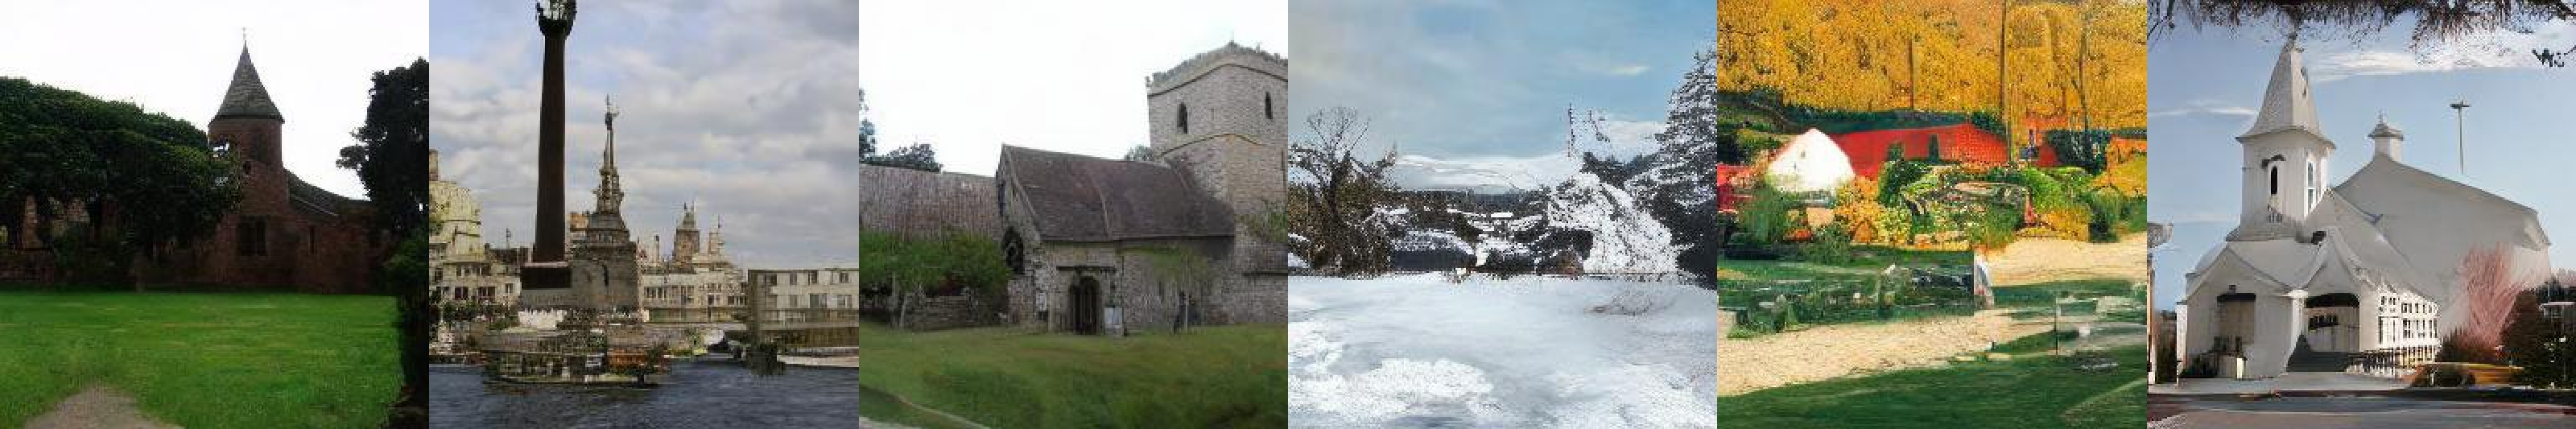
\includegraphics[width=\textwidth]{figures/church/w8a32.pdf} 
\caption*{Full Precision (Act) W8A32}
\label{appfig: church_w8a32}
\end{subfigure} \\

\begin{subfigure}{0.35\linewidth}
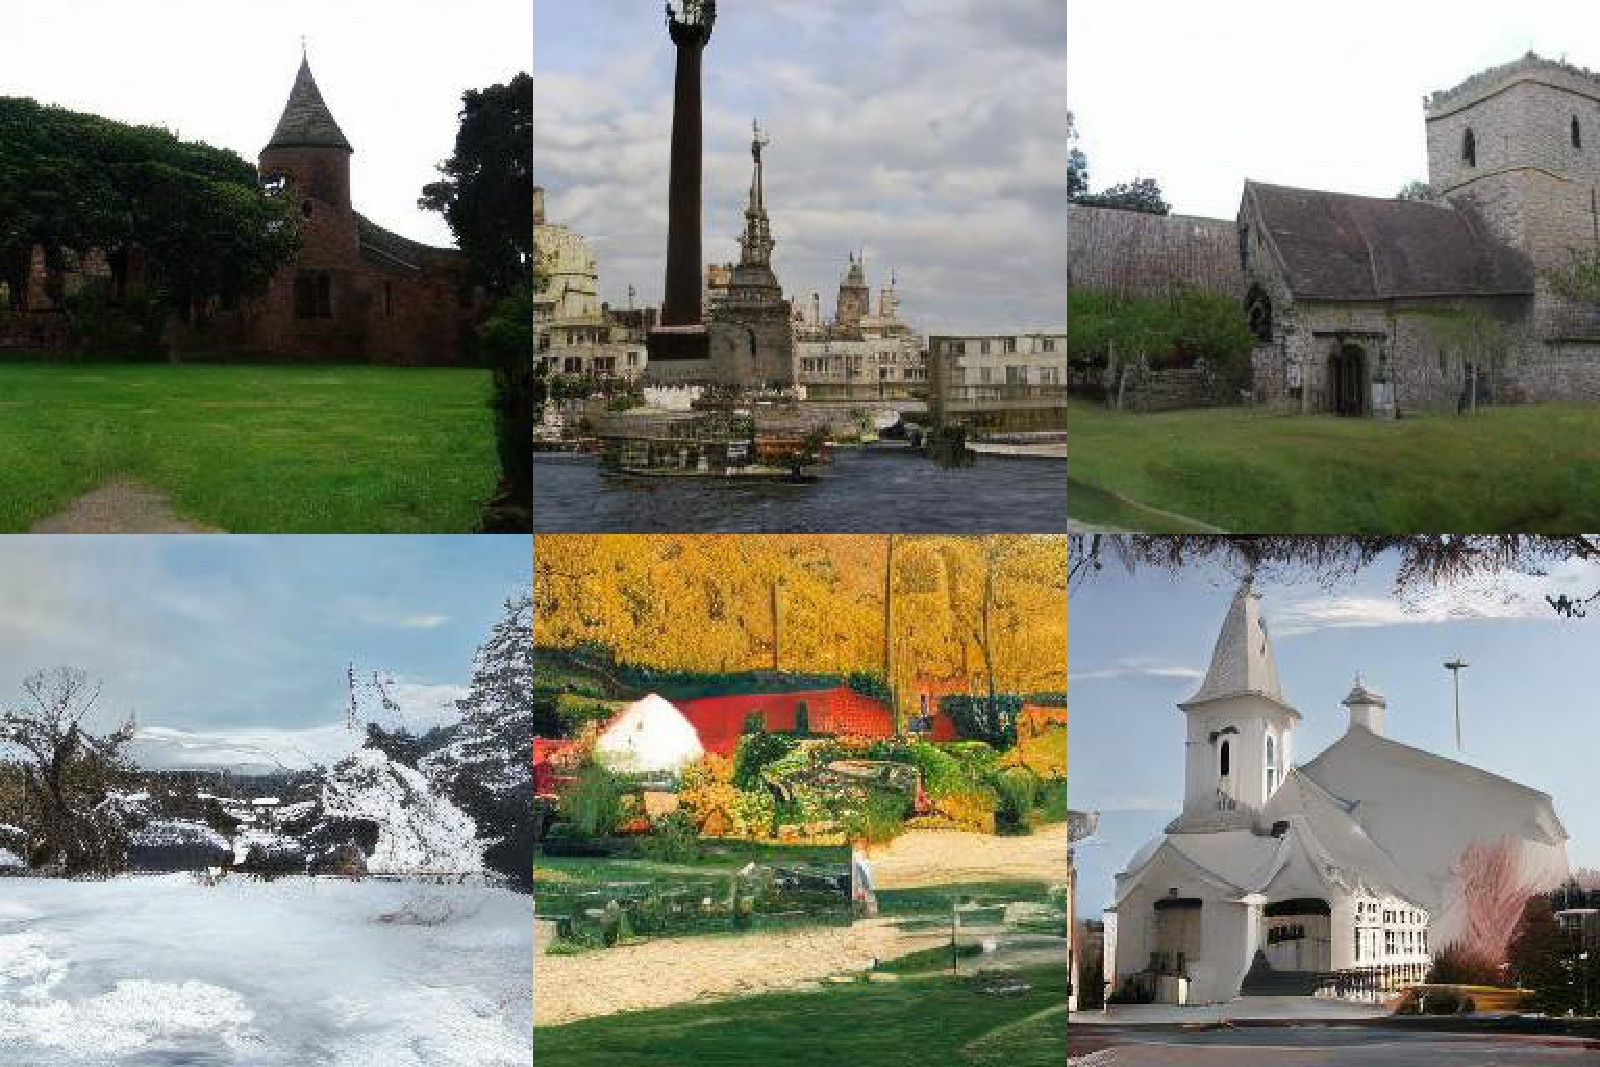
\includegraphics[width=\textwidth]{figures/church/w8a8.pdf}
\caption*{LCQ+MoDiff W8A8}
\label{appfig: church_w8a8}
\end{subfigure}
\hspace{0.5in}
\begin{subfigure}{0.35\linewidth}

\includegraphics[width=\textwidth]{figures/church/w8a8_rt.pdf}
\caption*{LCQ W8A8}
\label{appfig: church_w8a8_rt}
\end{subfigure} \\

\begin{subfigure}{0.35\linewidth}
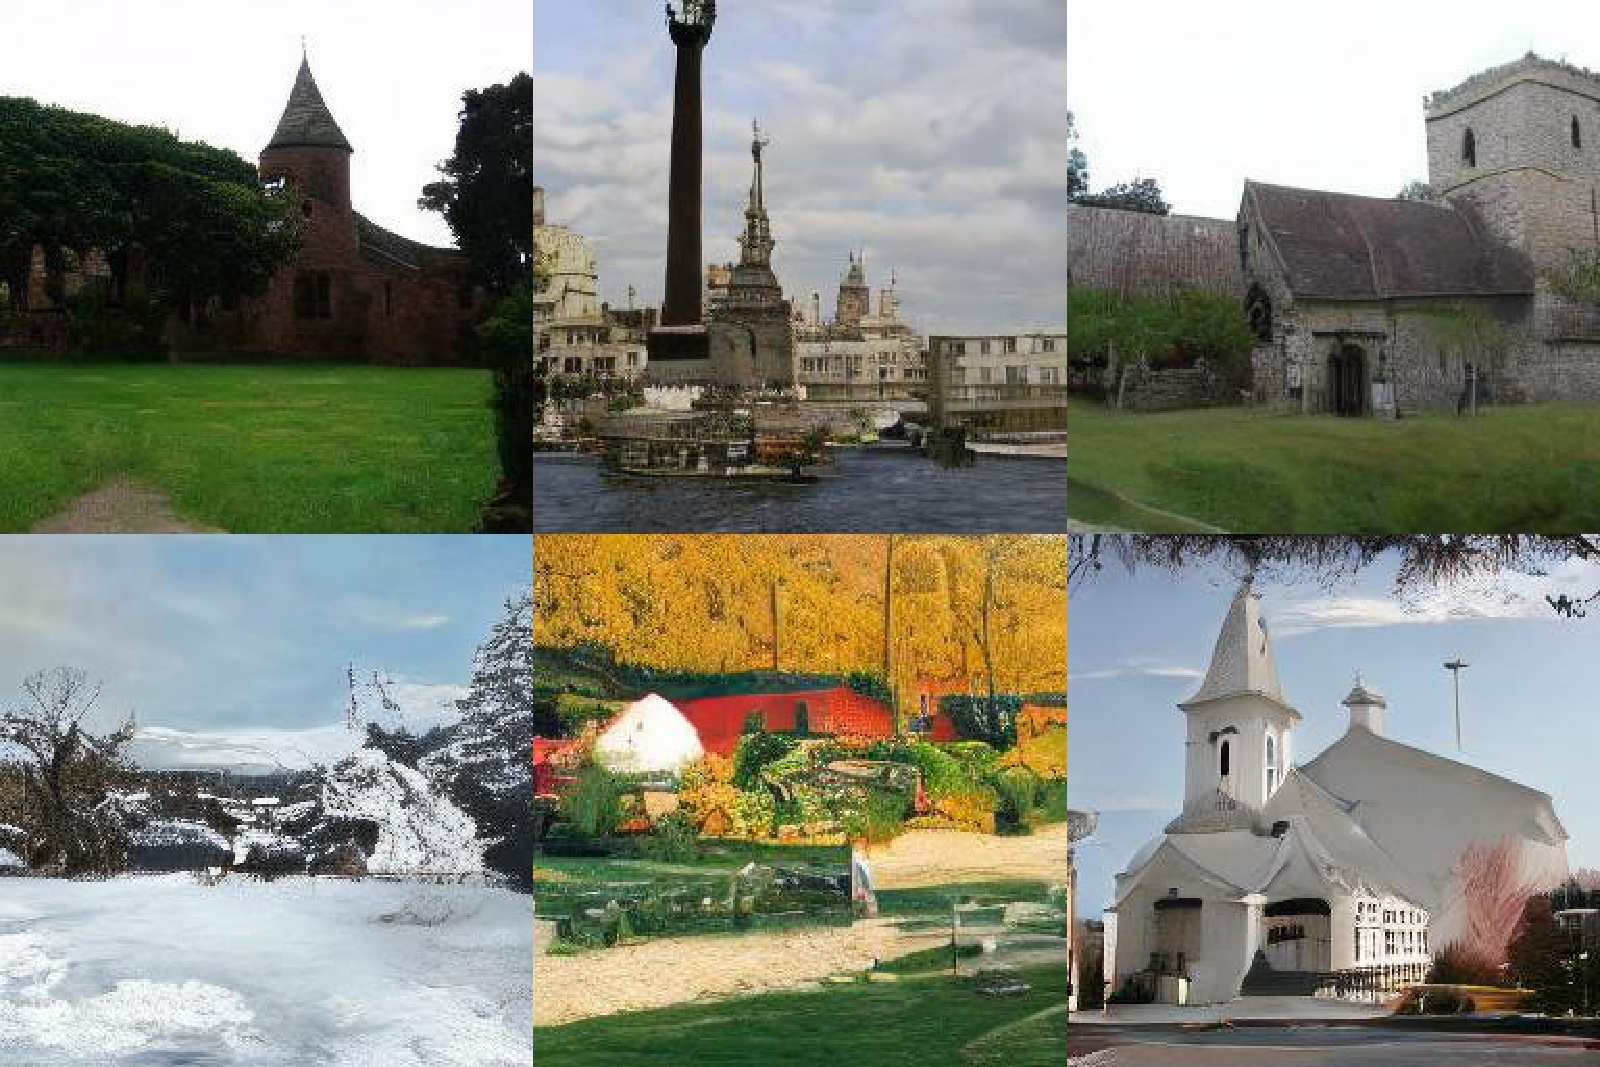
\includegraphics[width=\textwidth]{figures/church/w8a6.pdf}
\caption*{LCQ+MoDiff W8A6}
\label{appfig: church_w8a6}
\end{subfigure}
\hspace{0.5in}
\begin{subfigure}{0.35\linewidth}

\includegraphics[width=\textwidth]{figures/church/w8a6_rt.pdf}
\caption*{LCQ W8A6}
\label{appfig: church_w8a6_rt}
\end{subfigure} \\

\begin{subfigure}{0.35\linewidth}
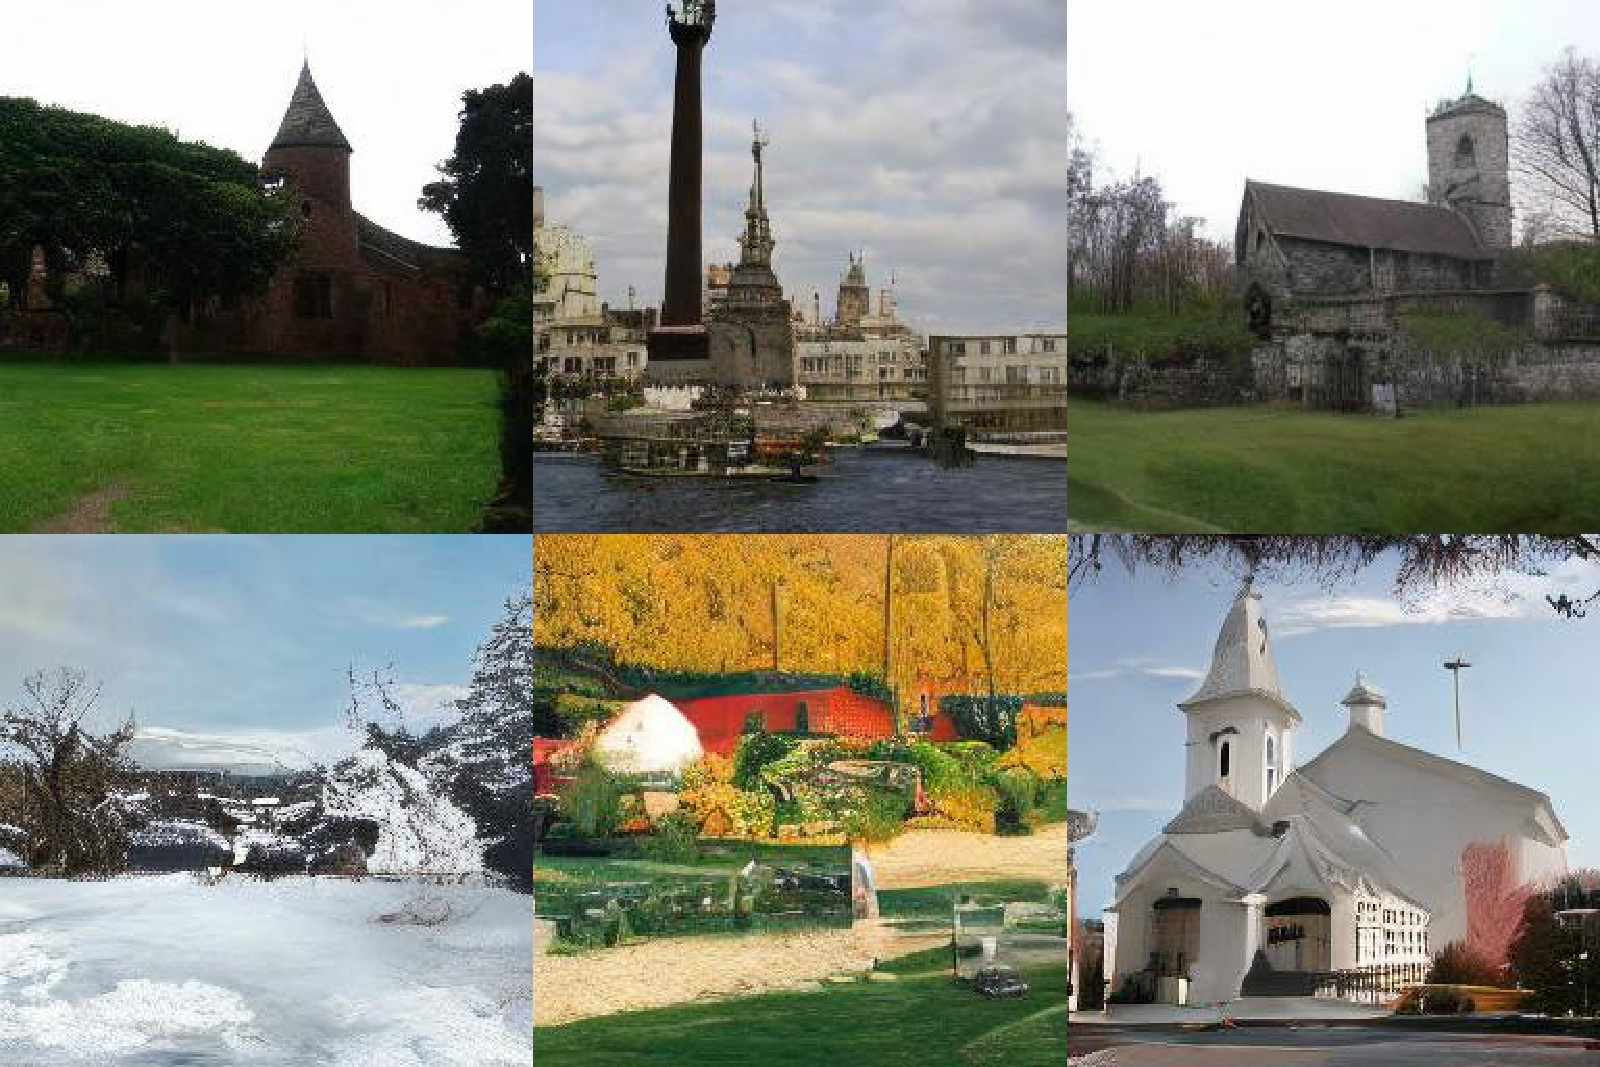
\includegraphics[width=\textwidth]{figures/church/w8a4.pdf}
\caption*{LCQ+MoDiff W8A4}
\label{appfig: church_w8a4}
\end{subfigure}
\hspace{0.5in}
\begin{subfigure}{0.35\linewidth}

\includegraphics[width=\textwidth]{figures/church/w8a4_rt.pdf}
\caption*{LCQ W8A4}
\label{appfig: church_w8a4_rt}
\end{subfigure} \\

\begin{subfigure}{0.35\linewidth}
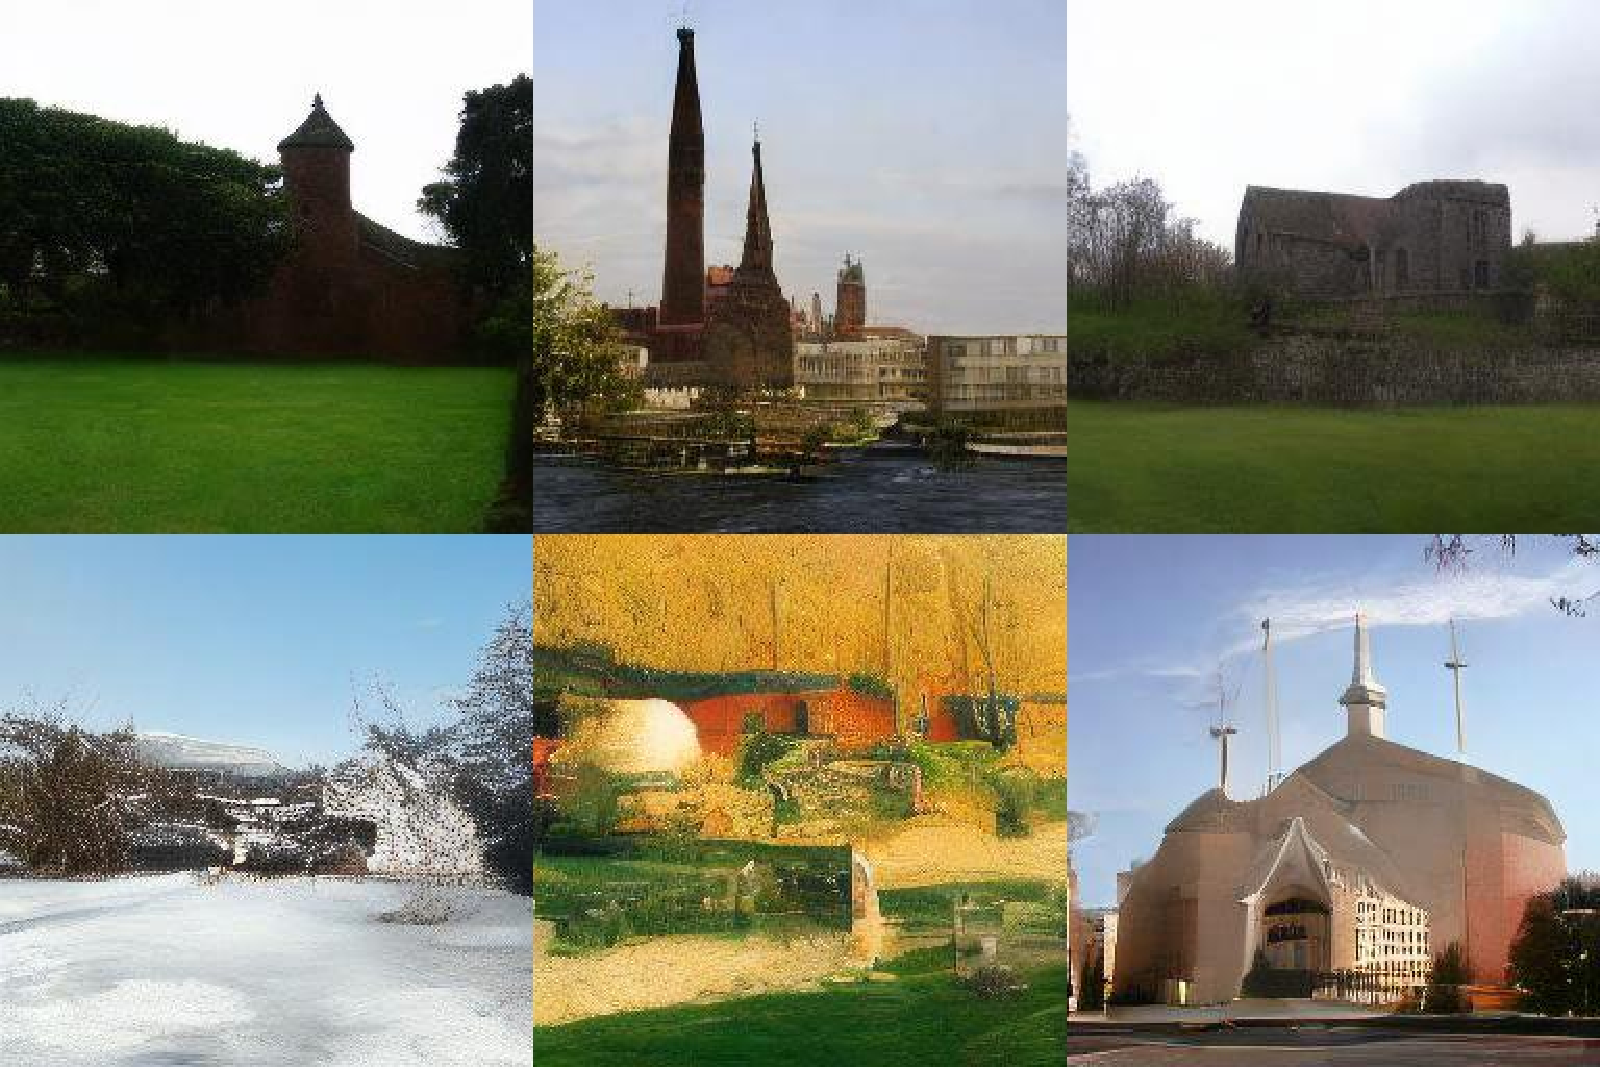
\includegraphics[width=\textwidth]{figures/church/w8a3.pdf}
\caption*{LCQ+MoDiff W8A3}
\label{appfig: church_w8a3}
\end{subfigure}
\hspace{0.5in}
\begin{subfigure}{0.35\linewidth}

\includegraphics[width=\textwidth]{figures/church/w8a2_rt.pdf}
\caption*{LCQ W8A3}
\label{appfig: church_w8a3_rt}
\end{subfigure}

\caption{Visualization of LSUN-Churches $256\times256$ generated using LCQ and LCQ+MoDiff under 8-bit weight quantization precisions.}
\label{appfig:visual_church_w8}
\end{figure*}

\begin{figure*}[ht!]
\center
\begin{subfigure}{0.9\linewidth}
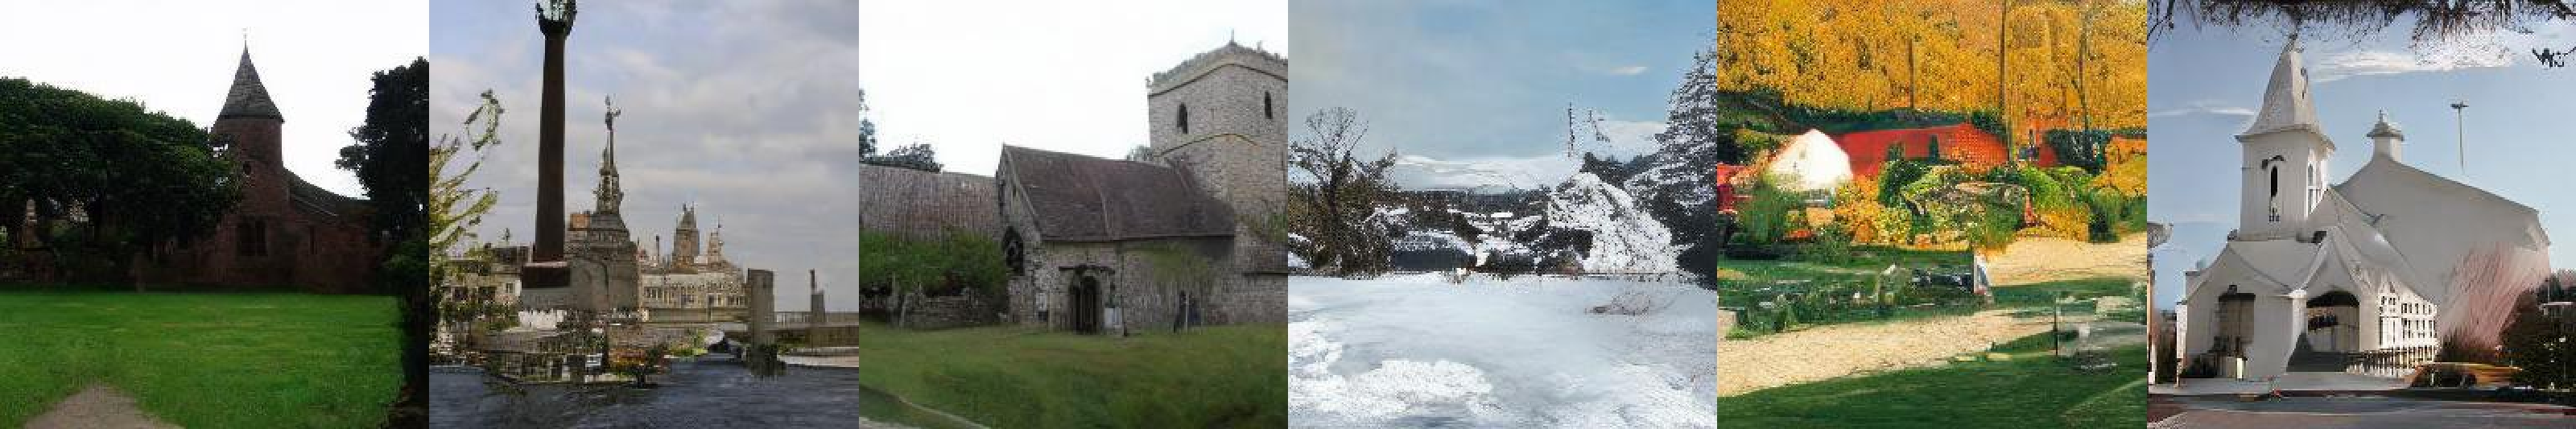
\includegraphics[width=\textwidth]{figures/church/w4a32.pdf} 
\caption*{Full Precision (Act) W4A32}
\label{appfig: church_w4a32}
\end{subfigure} \\

\begin{subfigure}{0.35\linewidth}
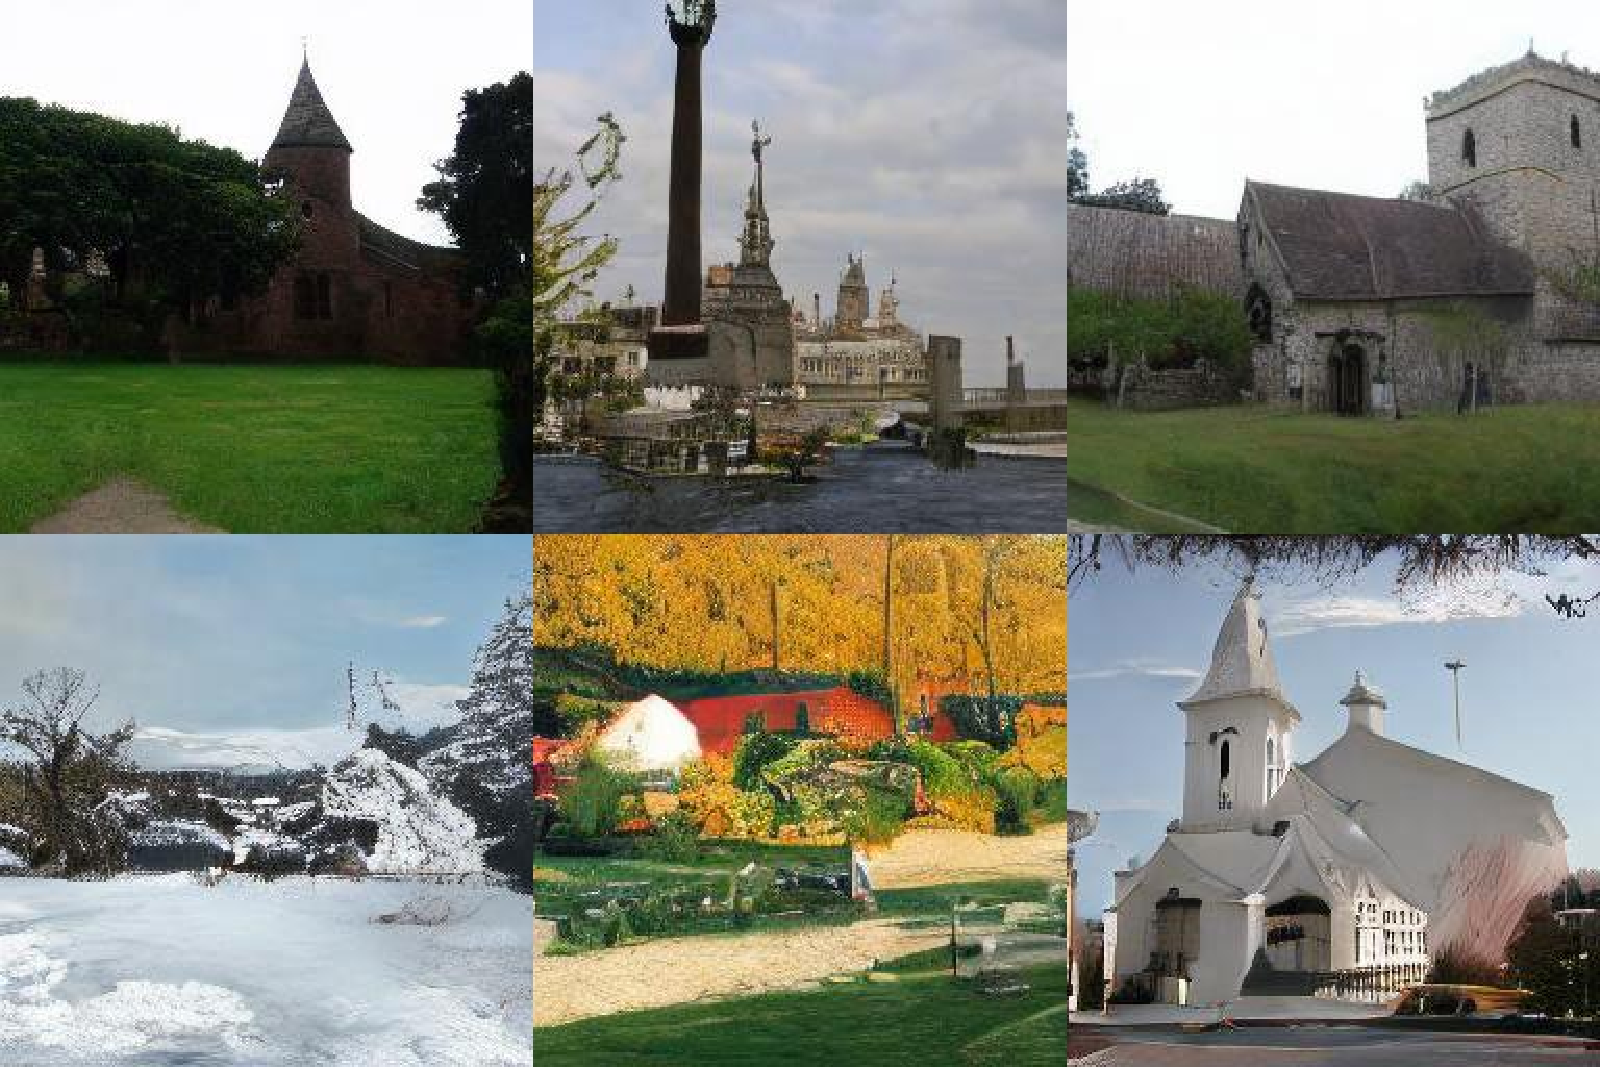
\includegraphics[width=\textwidth]{figures/church/w4a8.pdf}
\caption*{LCQ+MoDiff W4A8}
\label{appfig: church_w4a8}
\end{subfigure}
\hspace{0.5in}
\begin{subfigure}{0.35\linewidth}

\includegraphics[width=\textwidth]{figures/church/w4a8_rt.pdf}
\caption*{LCQ W4A8}
\label{appfig: church_w4a8_rt}
\end{subfigure} \\

\begin{subfigure}{0.35\linewidth}
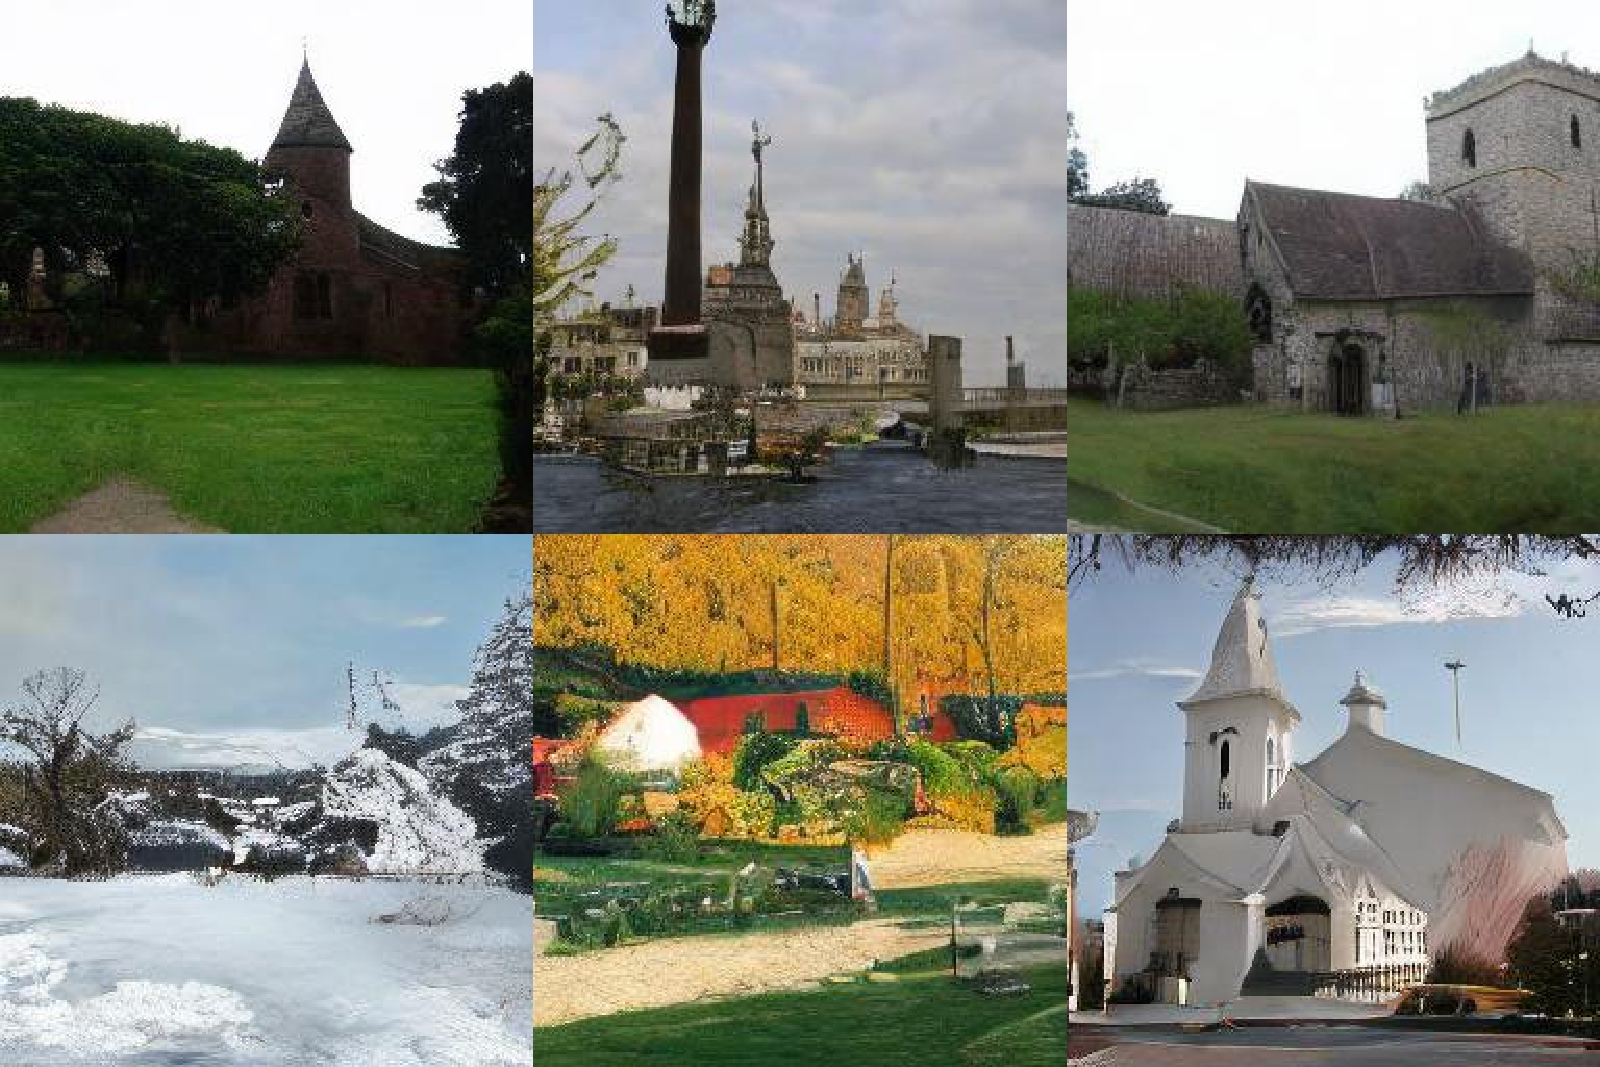
\includegraphics[width=\textwidth]{figures/church/w4a6.pdf}
\caption*{LCQ+MoDiff W4A6}
\label{appfig: church_w4a6}
\end{subfigure}
\hspace{0.5in}
\begin{subfigure}{0.35\linewidth}

\includegraphics[width=\textwidth]{figures/church/w4a6_rt.pdf}
\caption*{LCQ W4A6}
\label{appfig: church_w4a6_rt}
\end{subfigure} \\

\begin{subfigure}{0.35\linewidth}
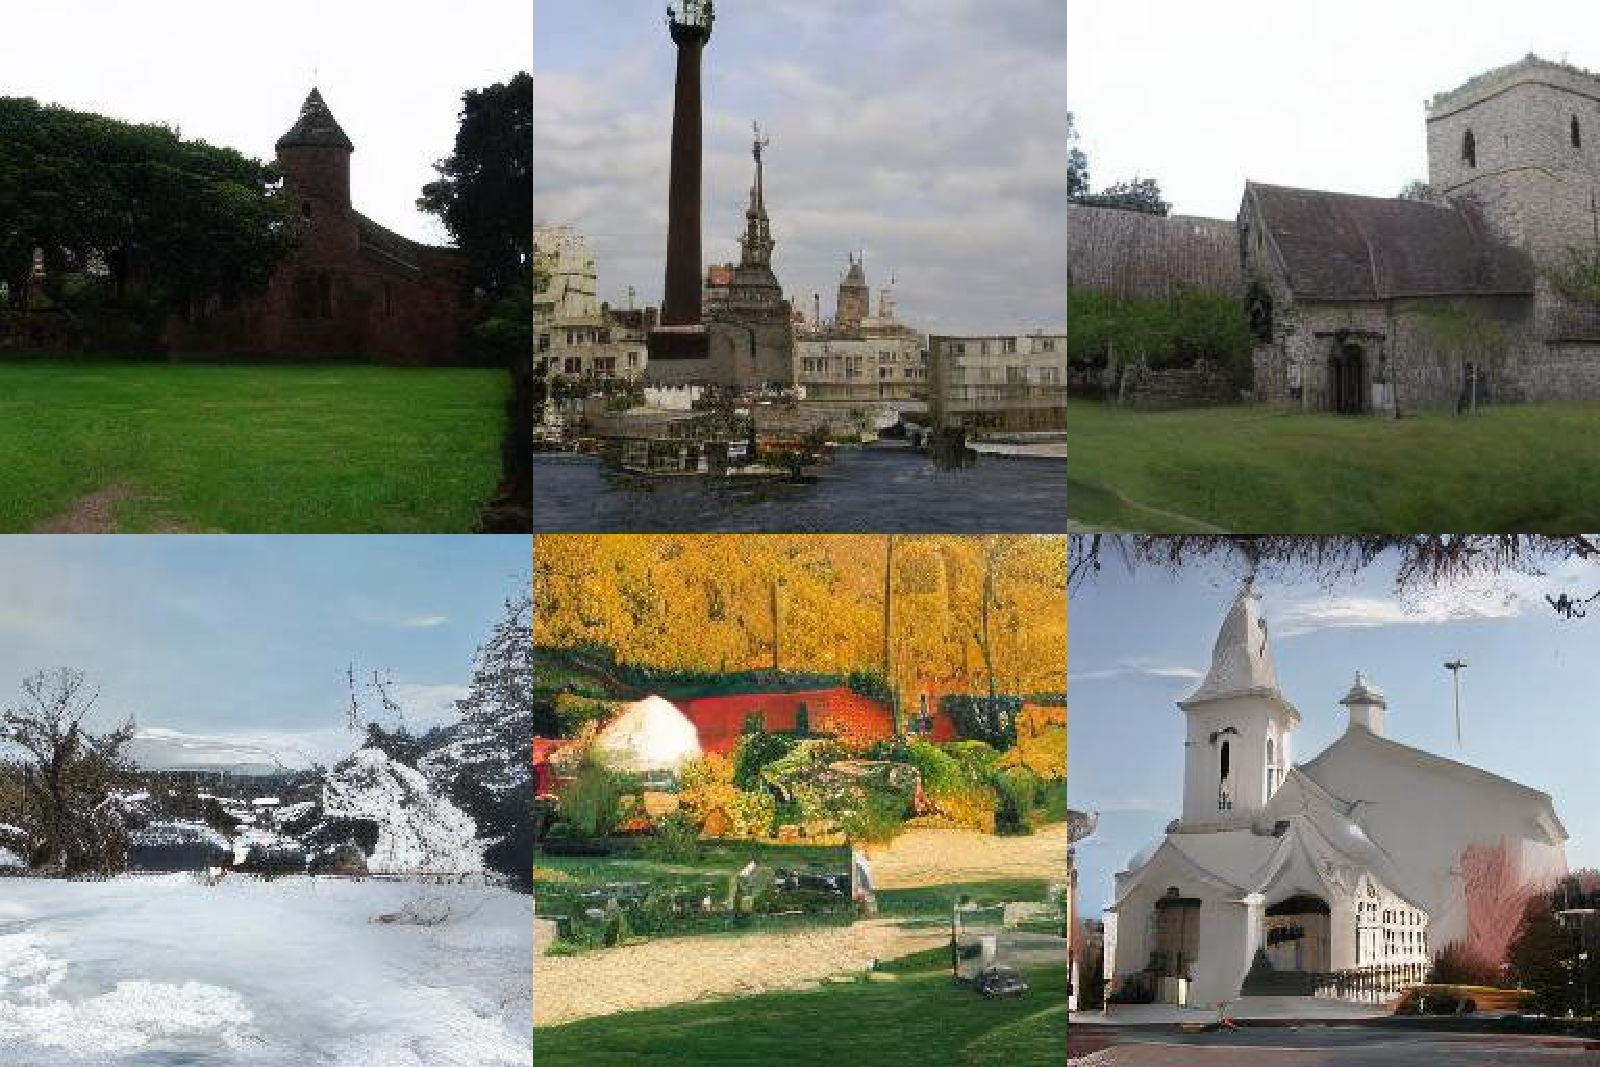
\includegraphics[width=\textwidth]{figures/church/w4a4.pdf}
\caption*{LCQ+MoDiff W4A4}
\label{appfig: church_w4a4}
\end{subfigure}
\hspace{0.5in}
\begin{subfigure}{0.35\linewidth}

\includegraphics[width=\textwidth]{figures/church/w4a4_rt.pdf}
\caption*{LCQ W4A4}
\label{appfig: church_w4a4_rt}
\end{subfigure} \\

\begin{subfigure}{0.35\linewidth}
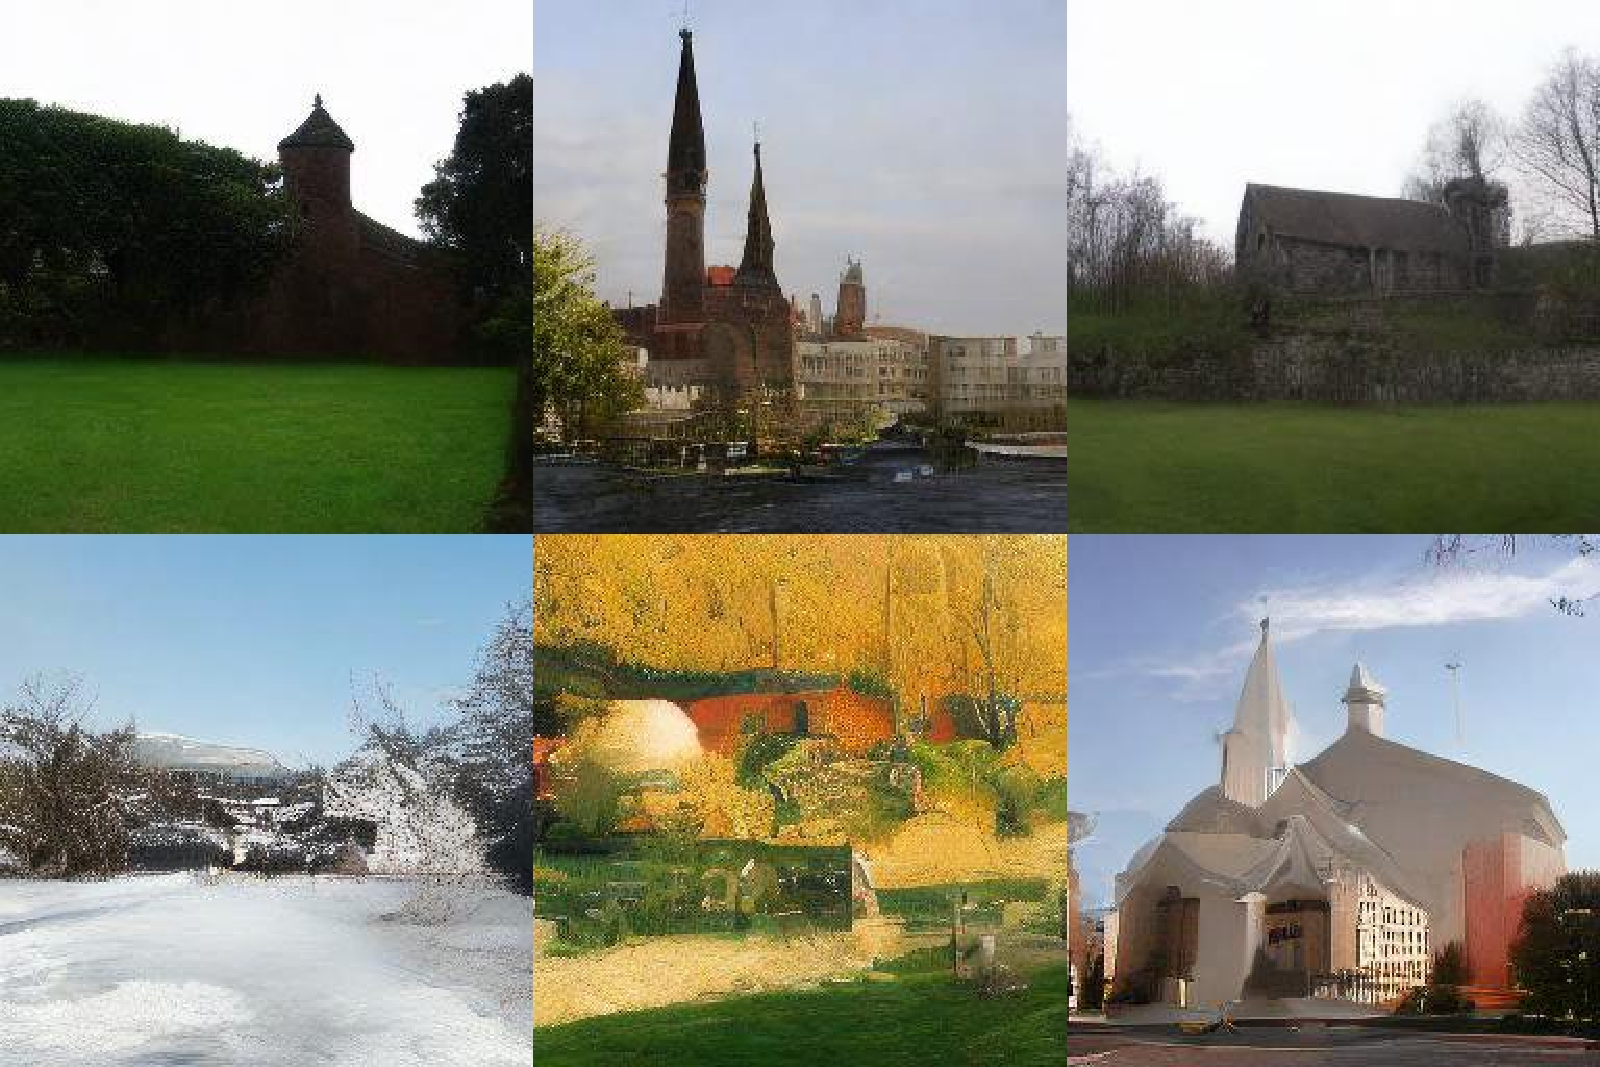
\includegraphics[width=\textwidth]{figures/church/w4a3.pdf}
\caption*{LCQ+MoDiff W4A3}
\label{appfig: church_w4a3}
\end{subfigure}
\hspace{0.5in}
\begin{subfigure}{0.35\linewidth}

\includegraphics[width=\textwidth]{figures/church/w4a2_rt.pdf}
\caption*{LCQ W4A3}
\label{appfig: church_w4a3_rt}
\end{subfigure}

\caption{Visualization of LSUN-Churches $256\times256$ generated using LCQ and LCQ+MoDiff under 4-bit weight quantization precisions.}
\label{appfig:visual_church_w4}
\end{figure*}

\begin{figure*}[ht!]
\center
\begin{subfigure}{0.9\linewidth}
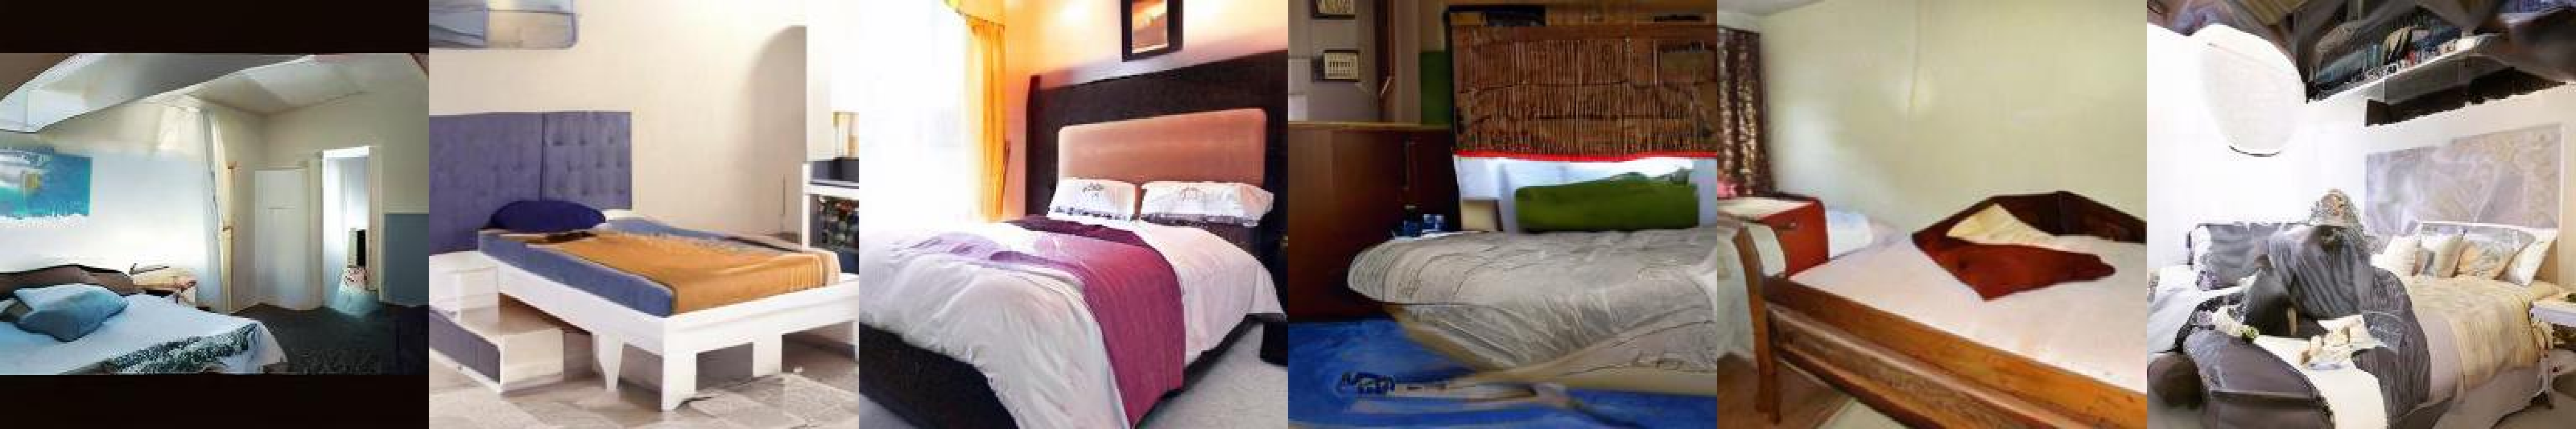
\includegraphics[width=\textwidth]{figures/bedroom/w8a32_e0.pdf} 
\caption*{Full Precision (Act) W8A32}
\label{appfig: bedroom_w8a32}
\end{subfigure} \\

\begin{subfigure}{0.35\linewidth}
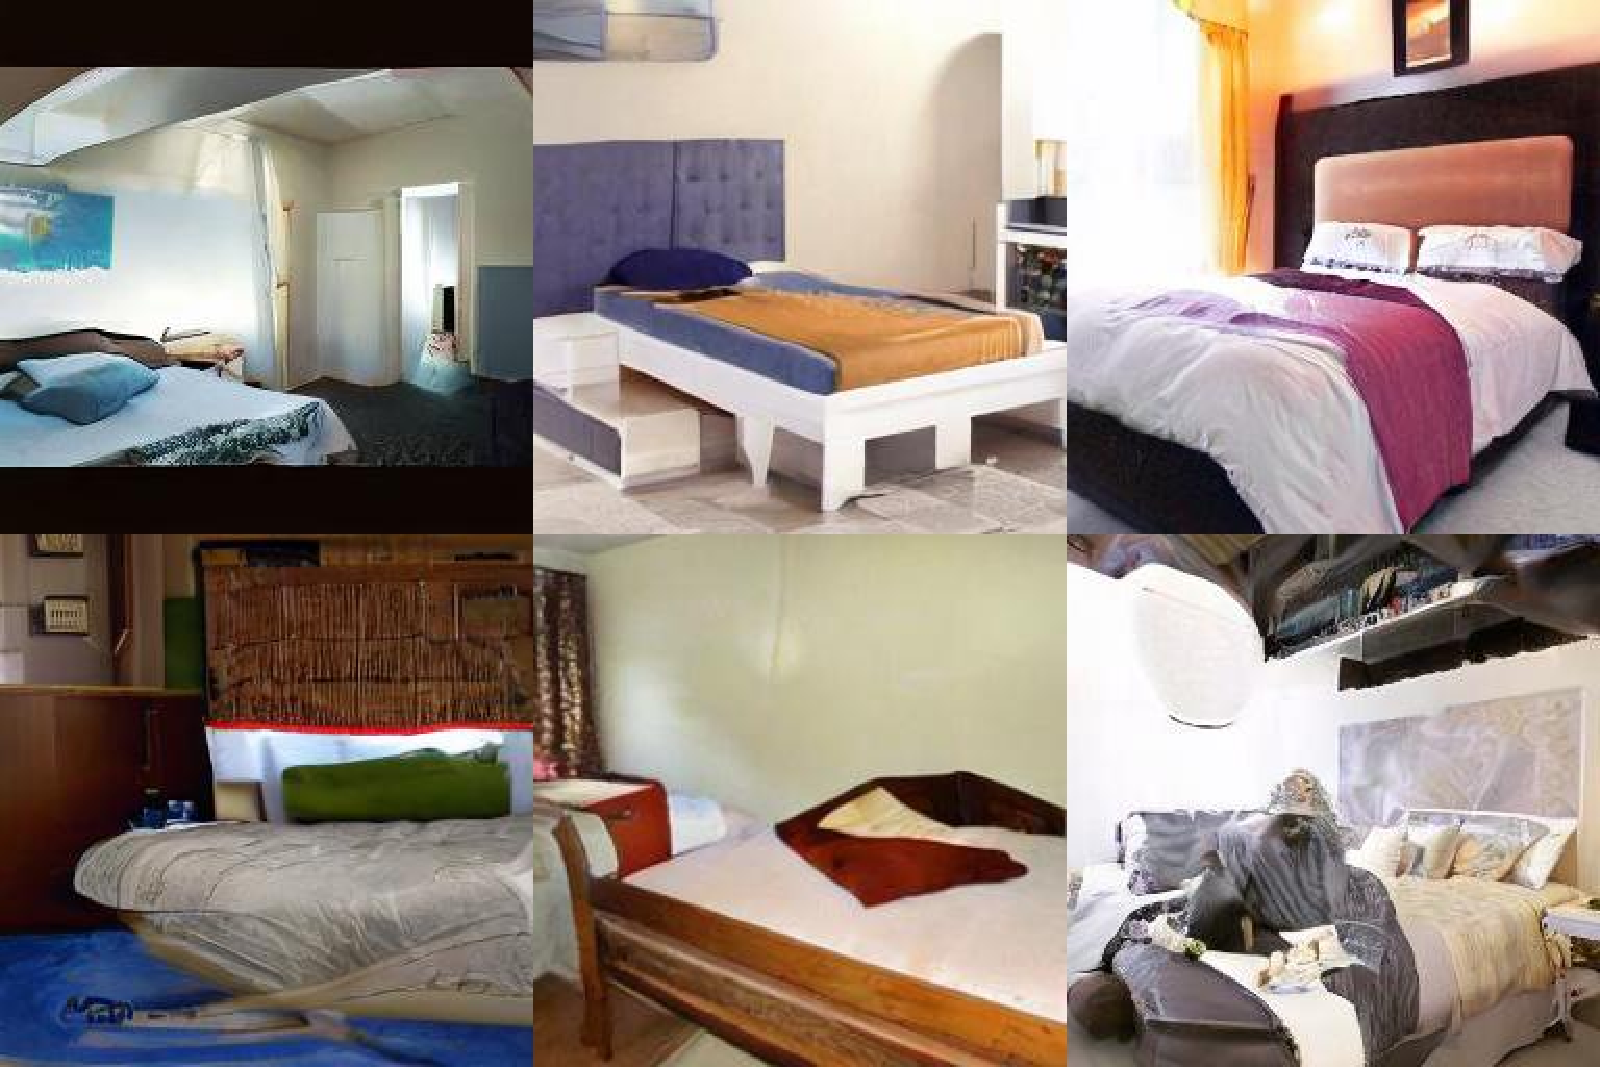
\includegraphics[width=\textwidth]{figures/bedroom/w8a8_e0.pdf}
\caption*{LCQ+MoDiff W8A8}
\label{appfig: bedroom_w8a8}
\end{subfigure}
\hspace{0.5in}
\begin{subfigure}{0.35\linewidth}
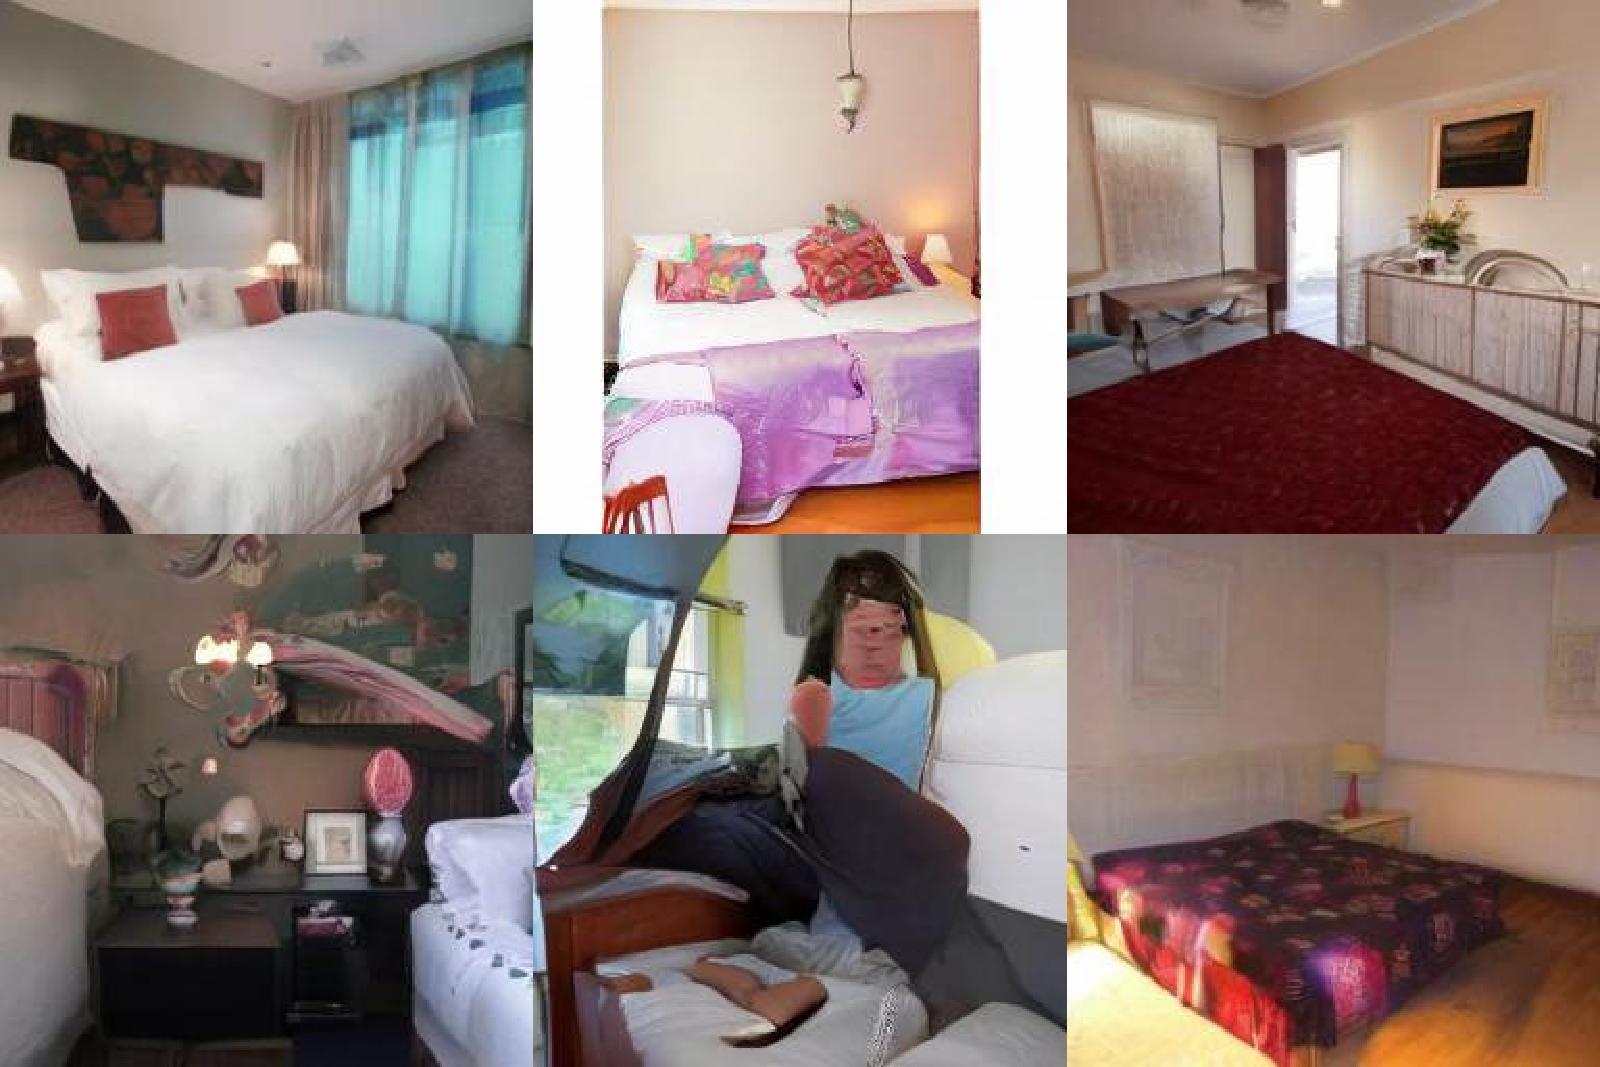
\includegraphics[width=\textwidth]{figures/bedroom/w8a8_rt.pdf}
\caption*{LCQ W8A8}
\label{appfig: bedroom_w8a8_rt}
\end{subfigure} \\

\begin{subfigure}{0.35\linewidth}
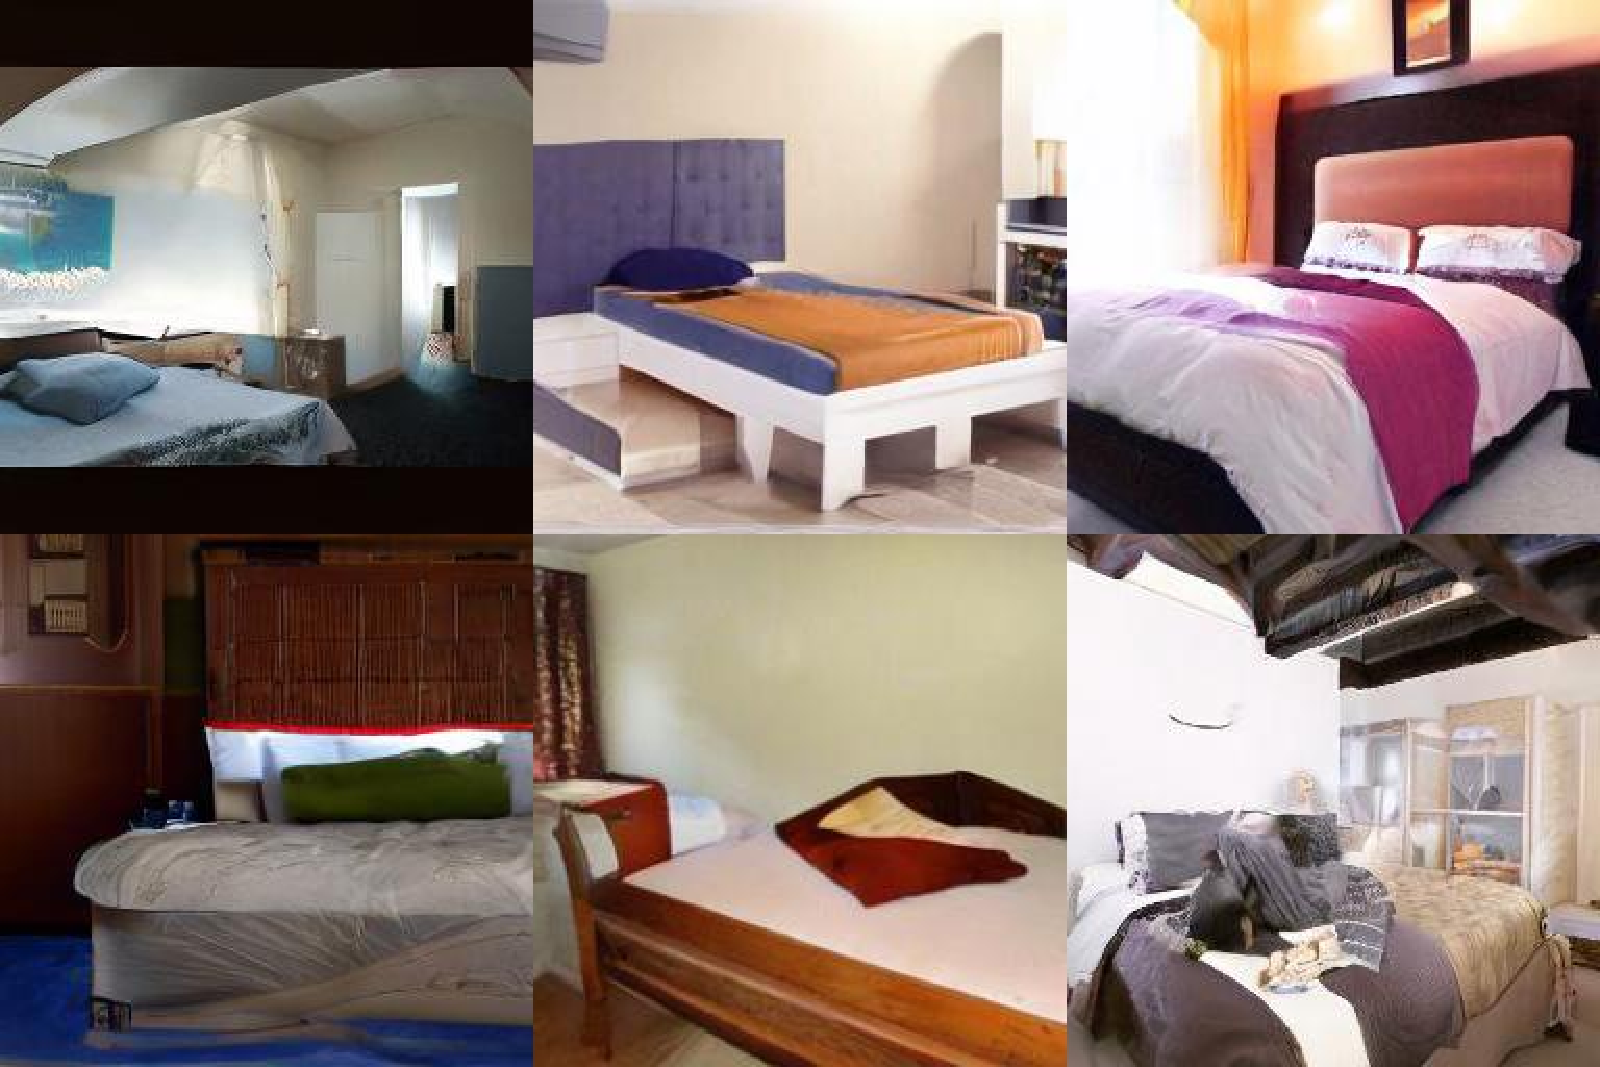
\includegraphics[width=\textwidth]{figures/bedroom/w8a6_e0.pdf}
\caption*{LCQ+MoDiff W8A6}
\label{appfig: bedroom_w8a6}
\end{subfigure}
\hspace{0.5in}
\begin{subfigure}{0.35\linewidth}
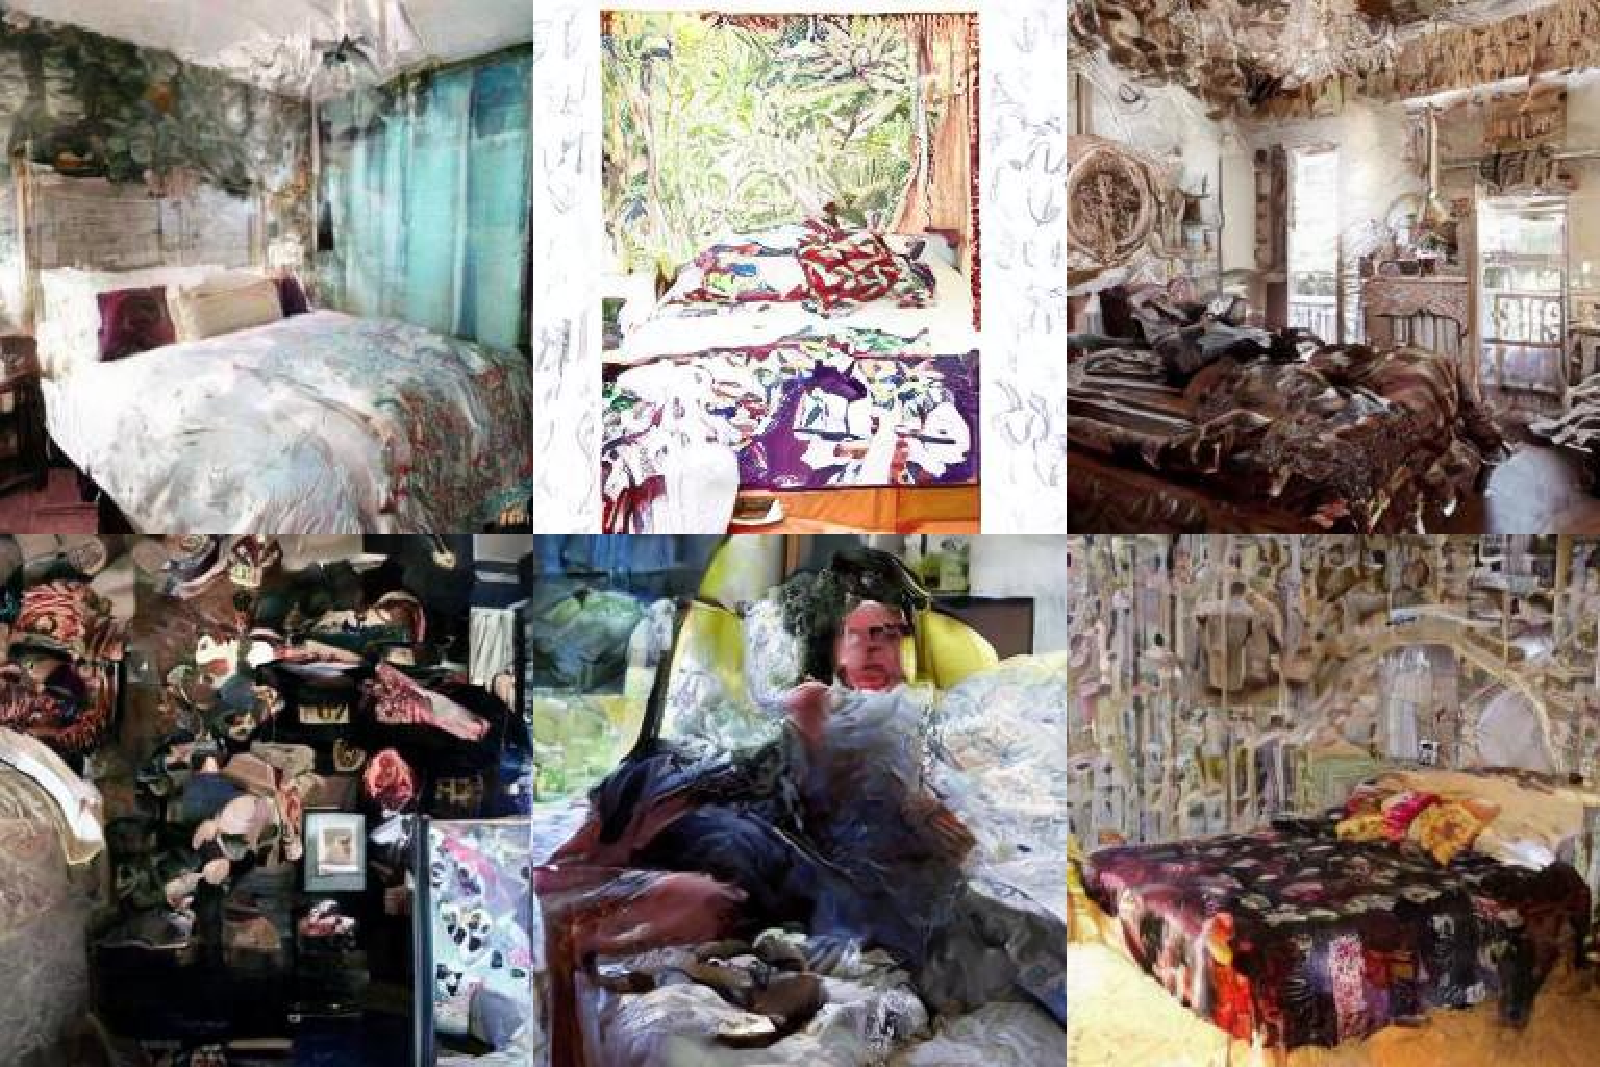
\includegraphics[width=\textwidth]{figures/bedroom/w8a6_rt.pdf}
\caption*{LCQ W8A6}
\label{appfig: bedroom_w8a6_rt}
\end{subfigure} \\

\begin{subfigure}{0.35\linewidth}
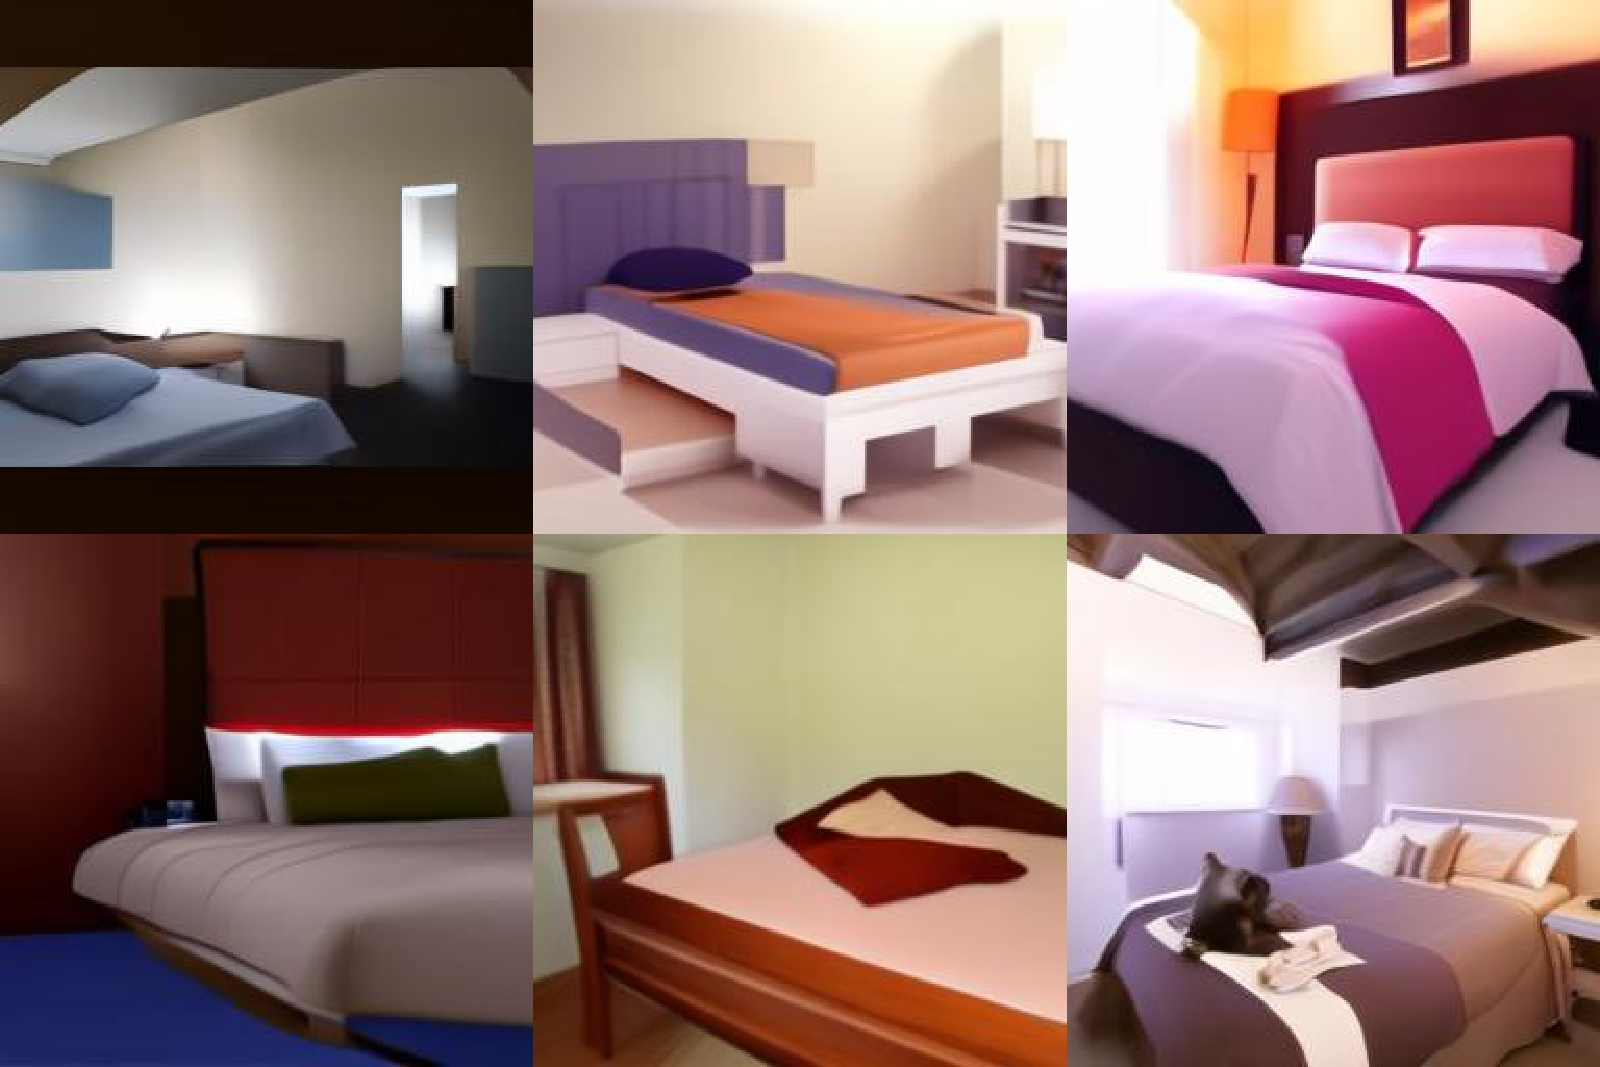
\includegraphics[width=\textwidth]{figures/bedroom/w8a4_e0.pdf}
\caption*{LCQ+MoDiff W8A4}
\label{appfig: bedroom_w8a4}
\end{subfigure}
\hspace{0.5in}
\begin{subfigure}{0.35\linewidth}
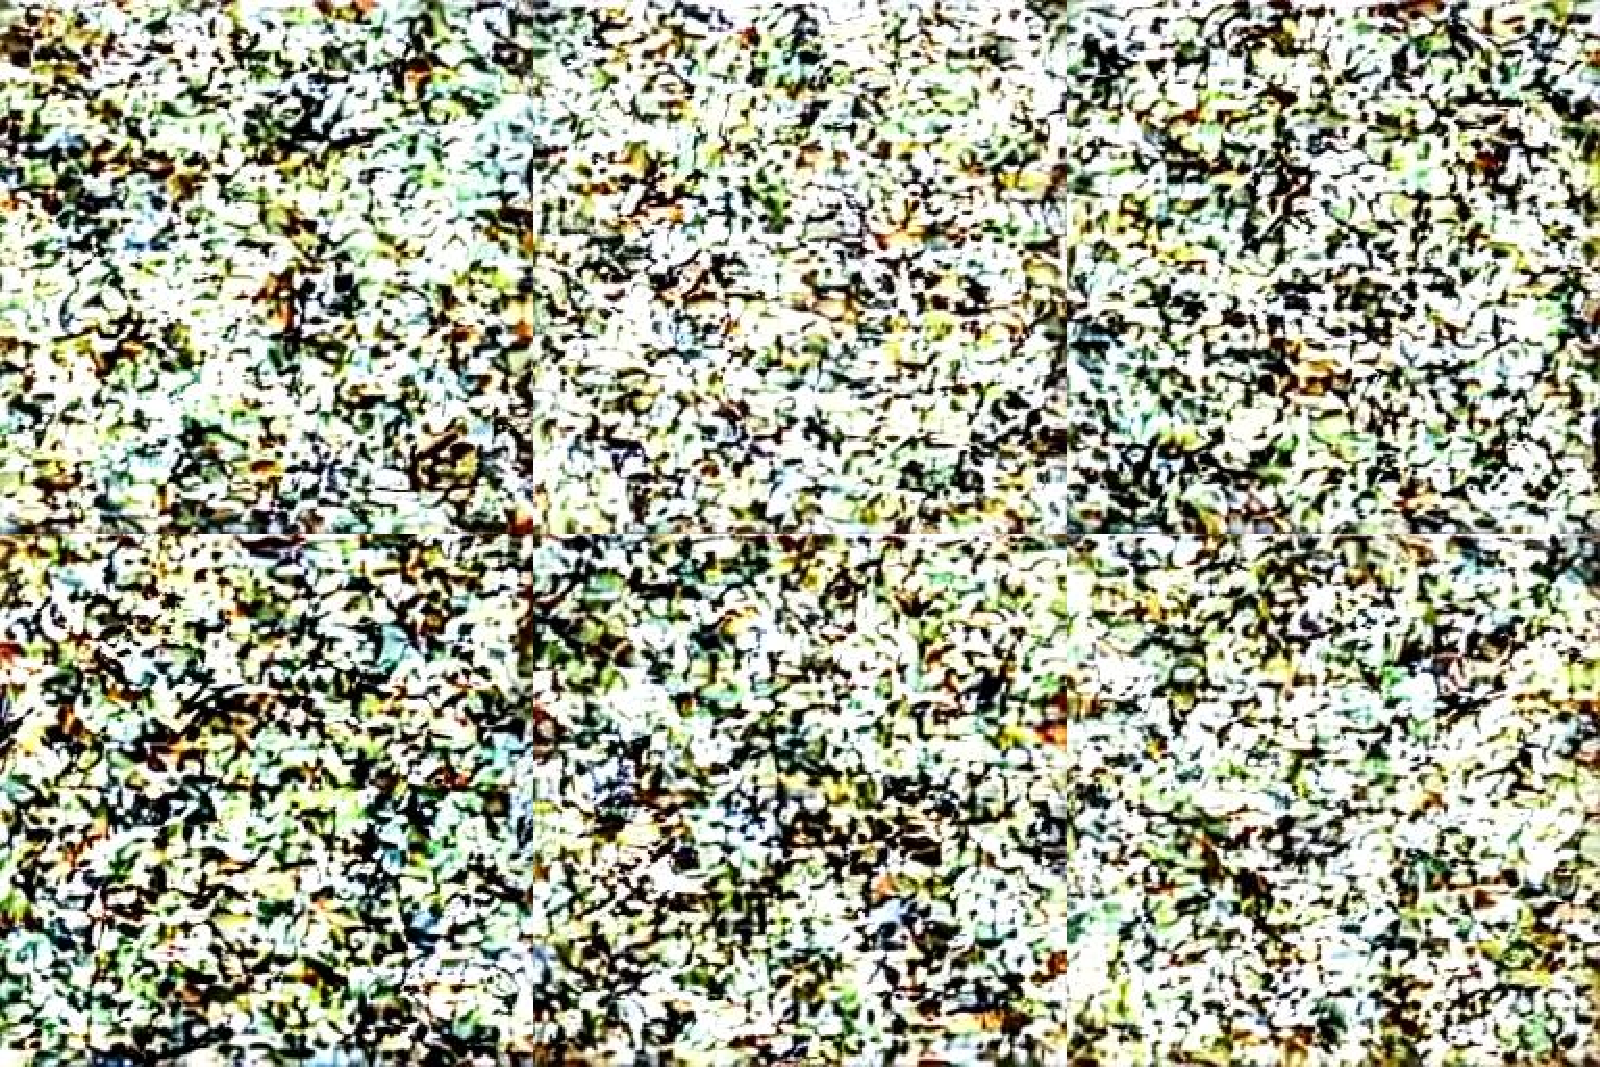
\includegraphics[width=\textwidth]{figures/bedroom/w8a4_rt.pdf}
\caption*{LCQ W8A4}
\label{appfig: bedroom_w8a4_rt}
\end{subfigure} 

\caption{Visualization of LSUN-bedrooms $256\times256$ generated using LCQ and LCQ+MoDiff under 8-bit weight quantization precisions.}
\label{appfig:visual_bedroom_w8}
\end{figure*}

\begin{figure*}[ht!]
\center
\begin{subfigure}{0.9\linewidth}
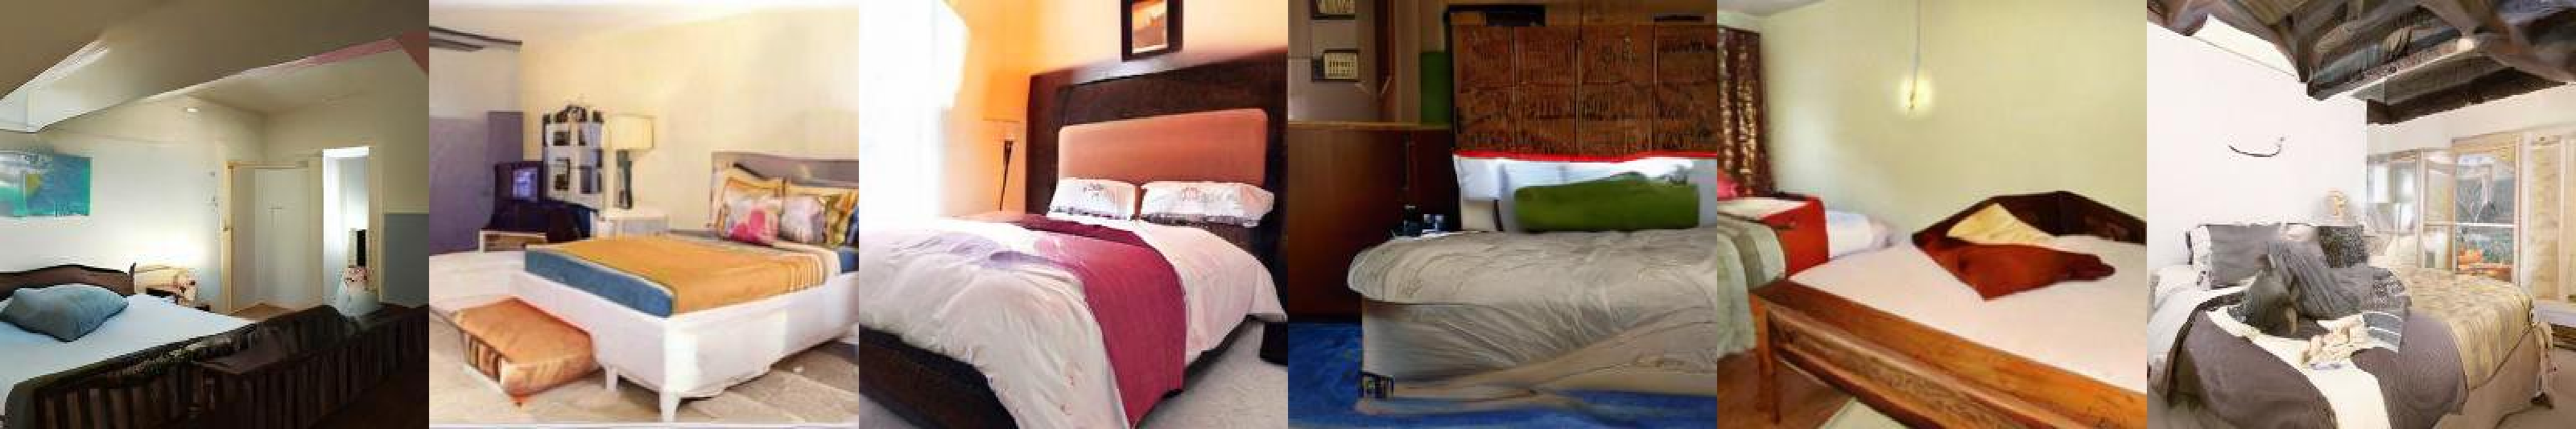
\includegraphics[width=\textwidth]{figures/bedroom/w4a32_e0.pdf} 
\caption*{Full Precision (Act) W4A32}
\label{appfig: bedroom_w4a32}
\end{subfigure} \\

\begin{subfigure}{0.35\linewidth}
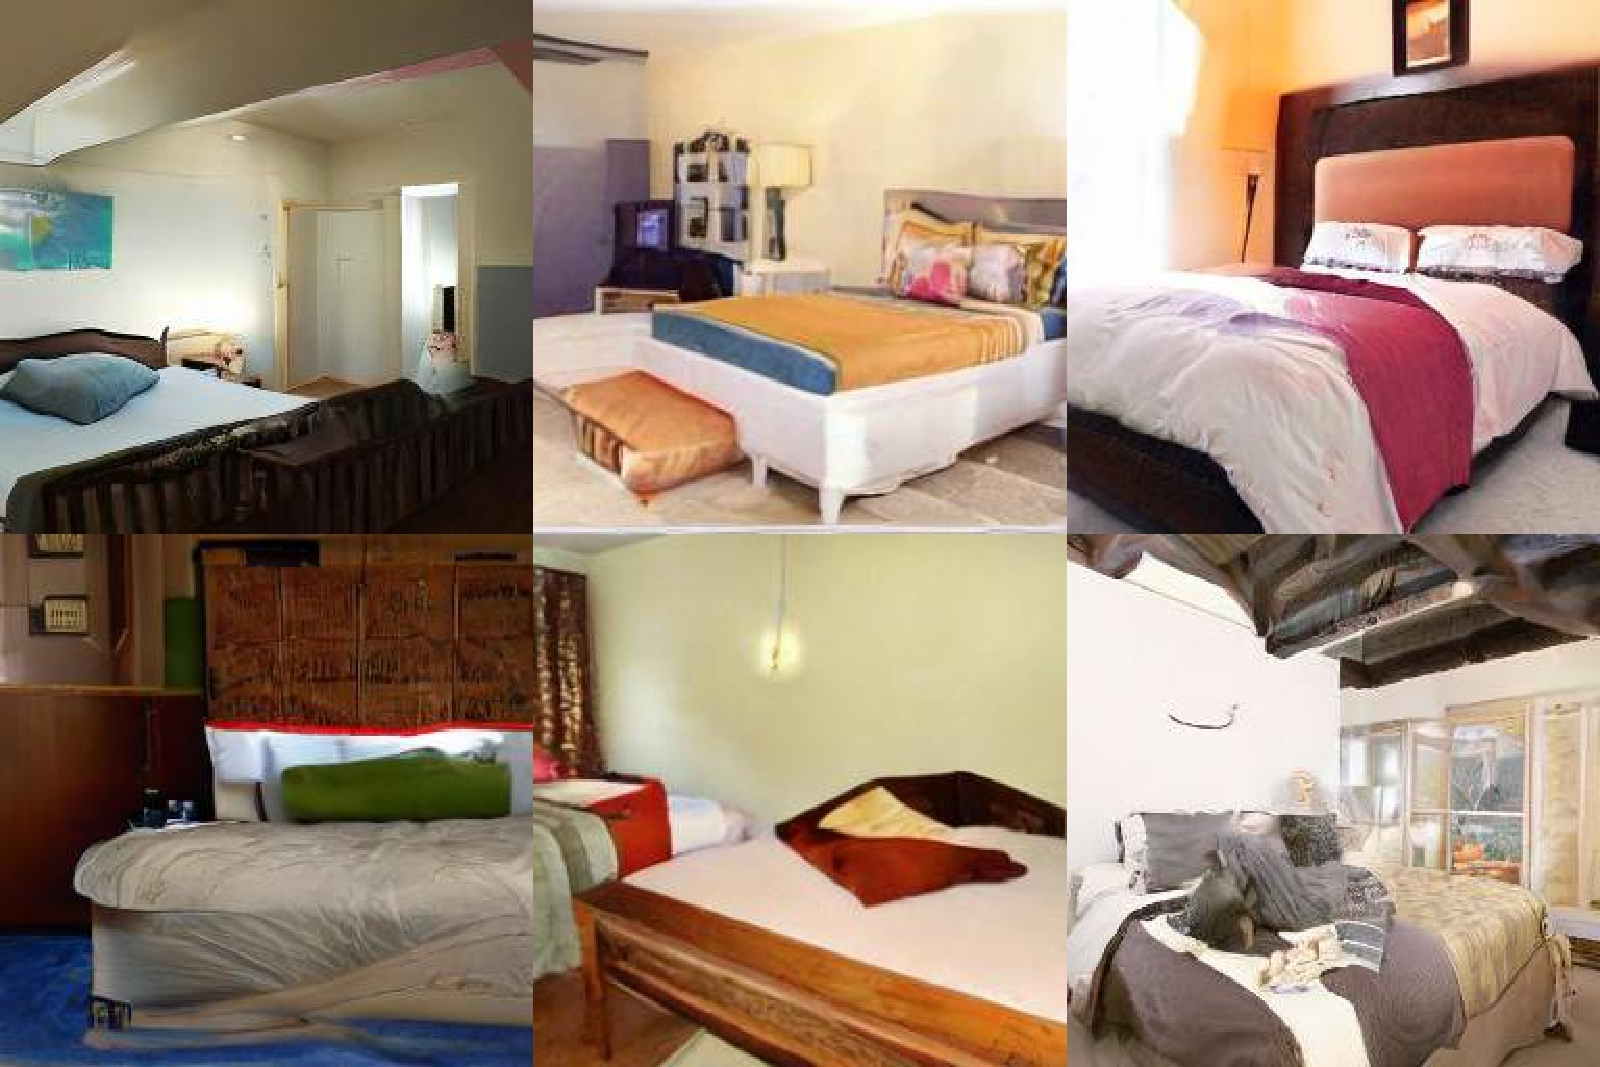
\includegraphics[width=\textwidth]{figures/bedroom/w4a8_e0.pdf}
\caption*{LCQ+MoDiff W4A8}
\label{appfig: bedroom_w4a8}
\end{subfigure}
\hspace{0.5in}
\begin{subfigure}{0.35\linewidth}
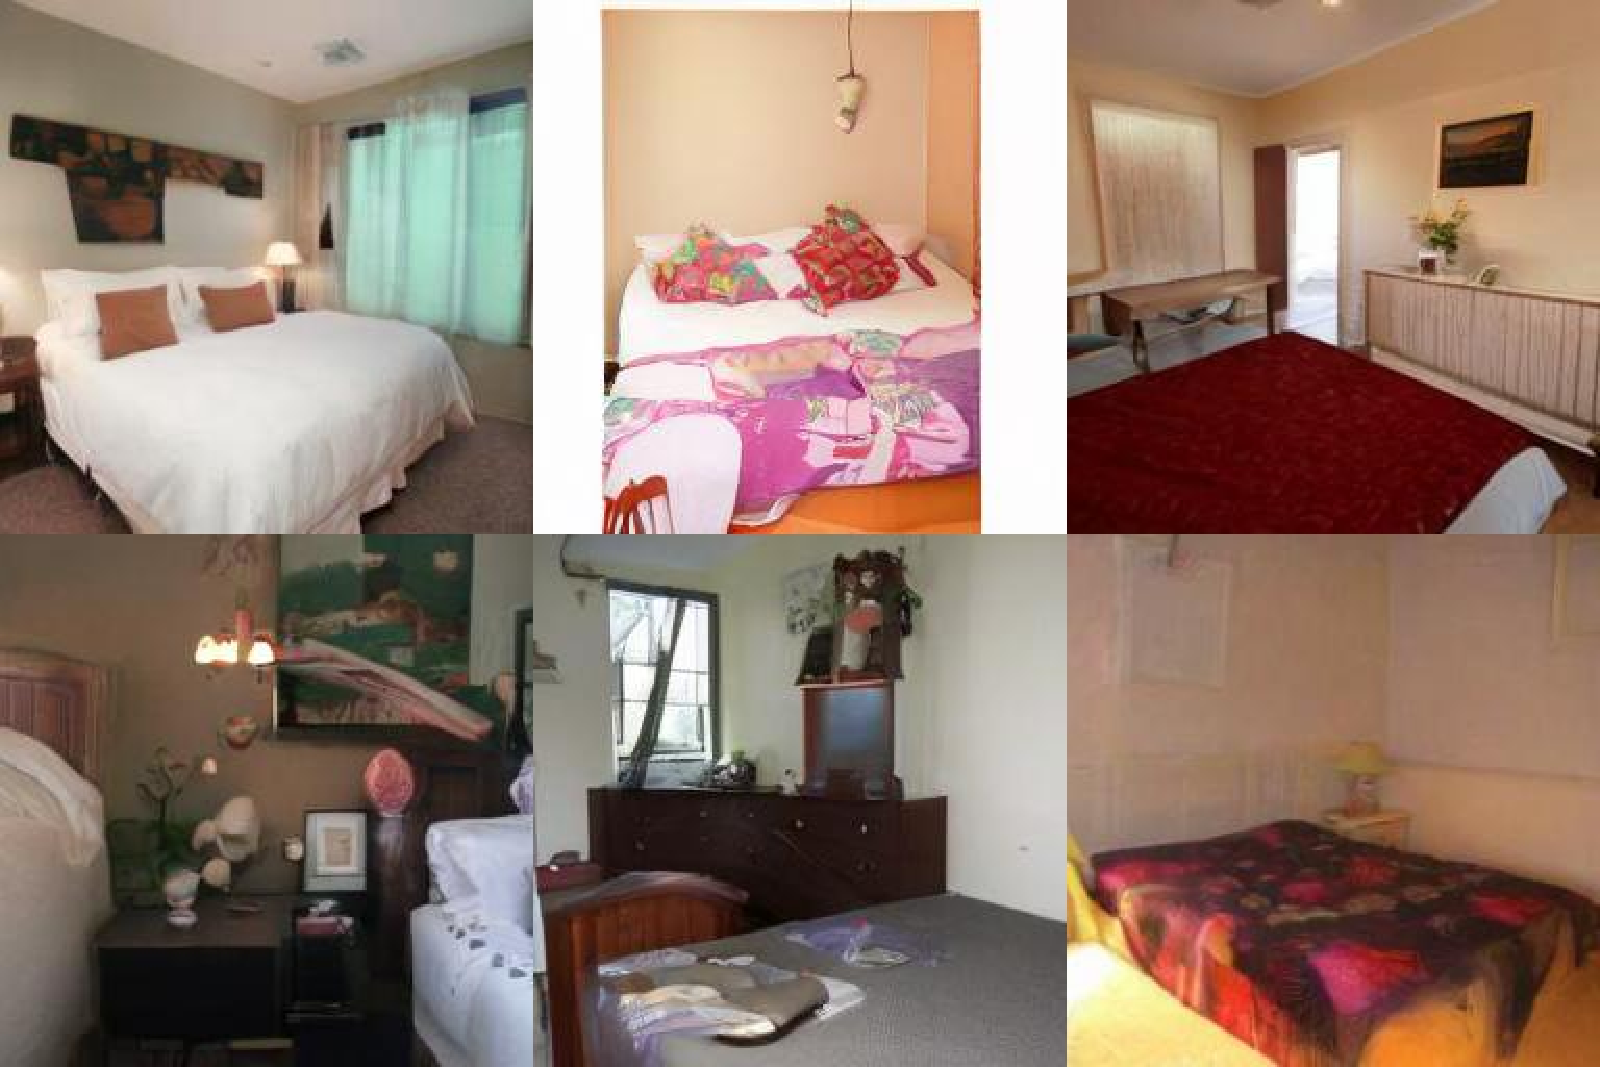
\includegraphics[width=\textwidth]{figures/bedroom/w4a8_rt.pdf}
\caption*{LCQ W4A8}
\label{appfig: bedroom_w4a8_rt}
\end{subfigure} \\

\begin{subfigure}{0.35\linewidth}
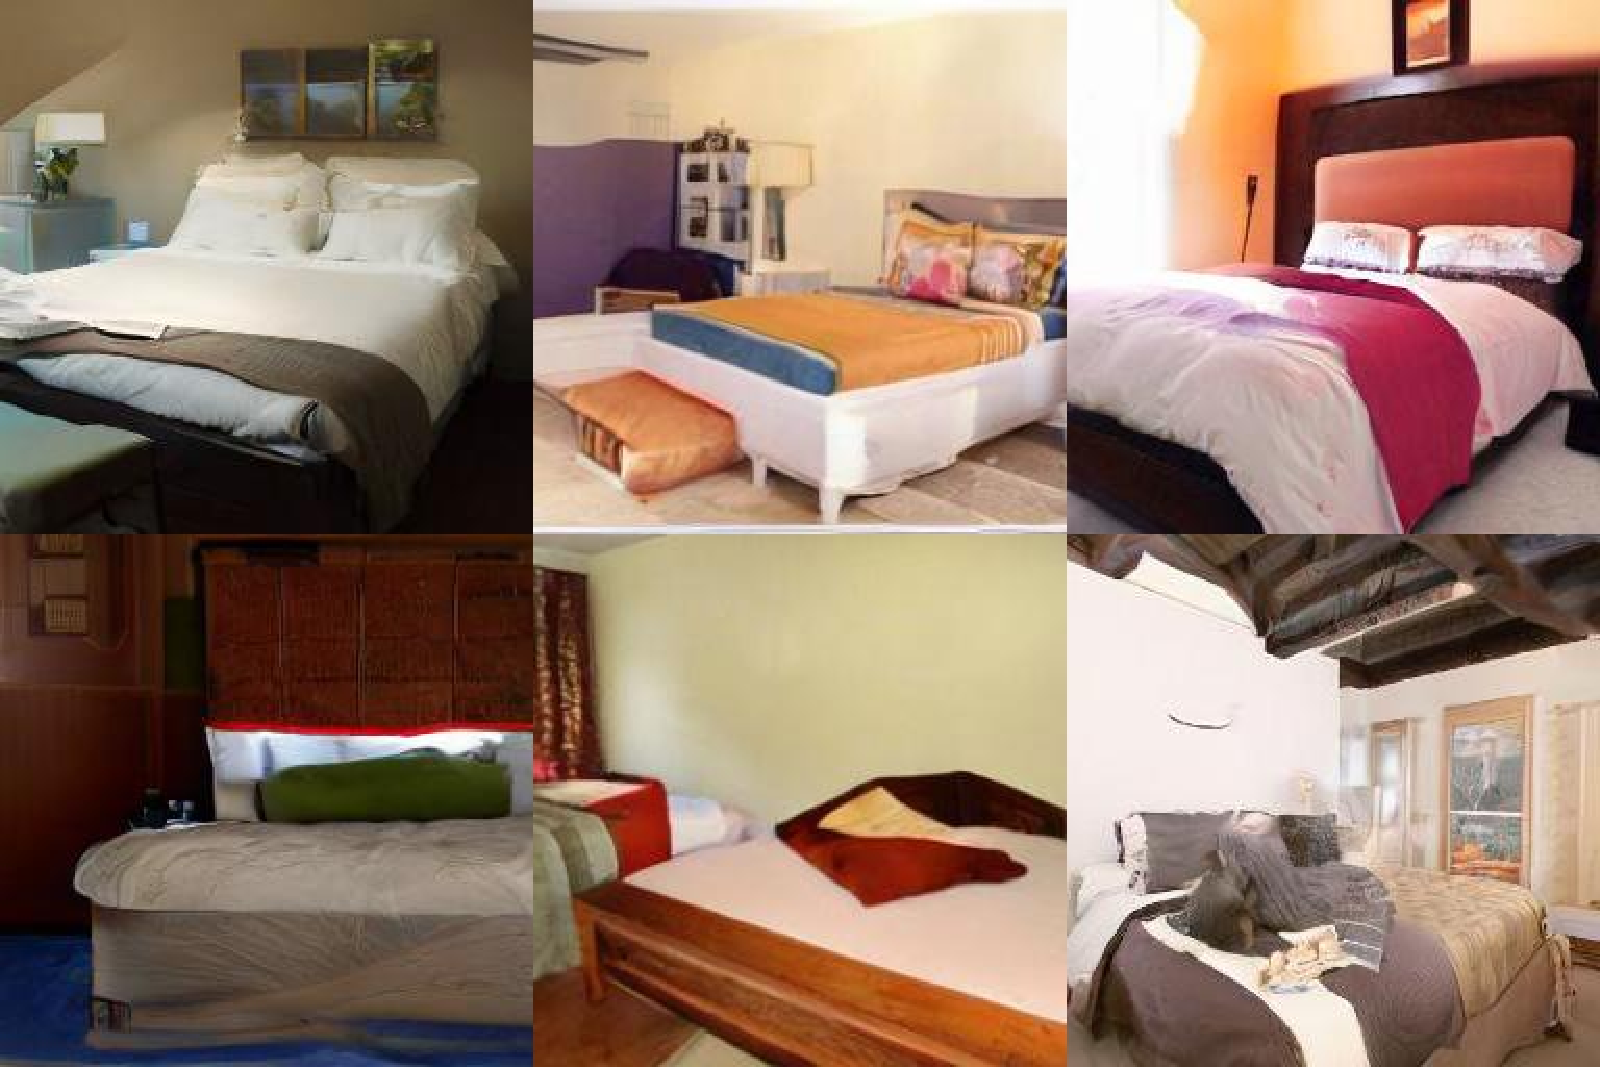
\includegraphics[width=\textwidth]{figures/bedroom/w4a6_e0.pdf}
\caption*{LCQ+MoDiff W4A6}
\label{appfig: bedroom_w4a6}
\end{subfigure}
\hspace{0.5in}
\begin{subfigure}{0.35\linewidth}
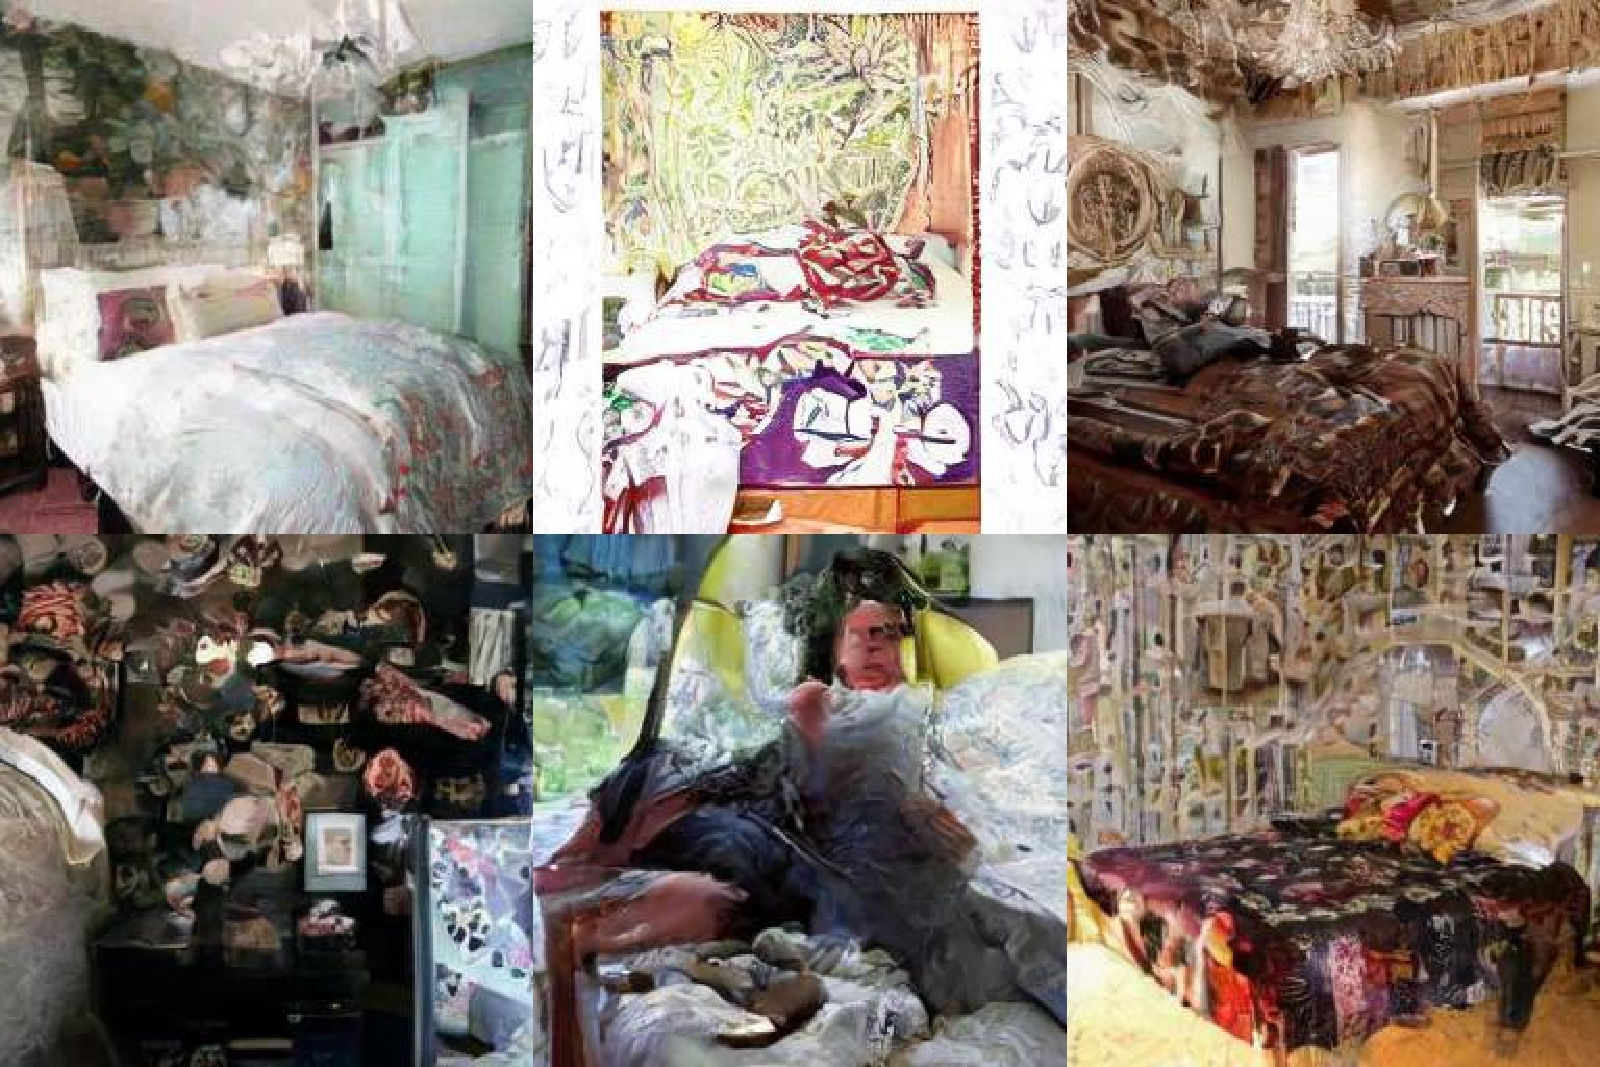
\includegraphics[width=\textwidth]{figures/bedroom/w4a6_rt.pdf}
\caption*{LCQ W4A6}
\label{appfig: bedroom_w4a6_rt}
\end{subfigure} \\

\begin{subfigure}{0.35\linewidth}
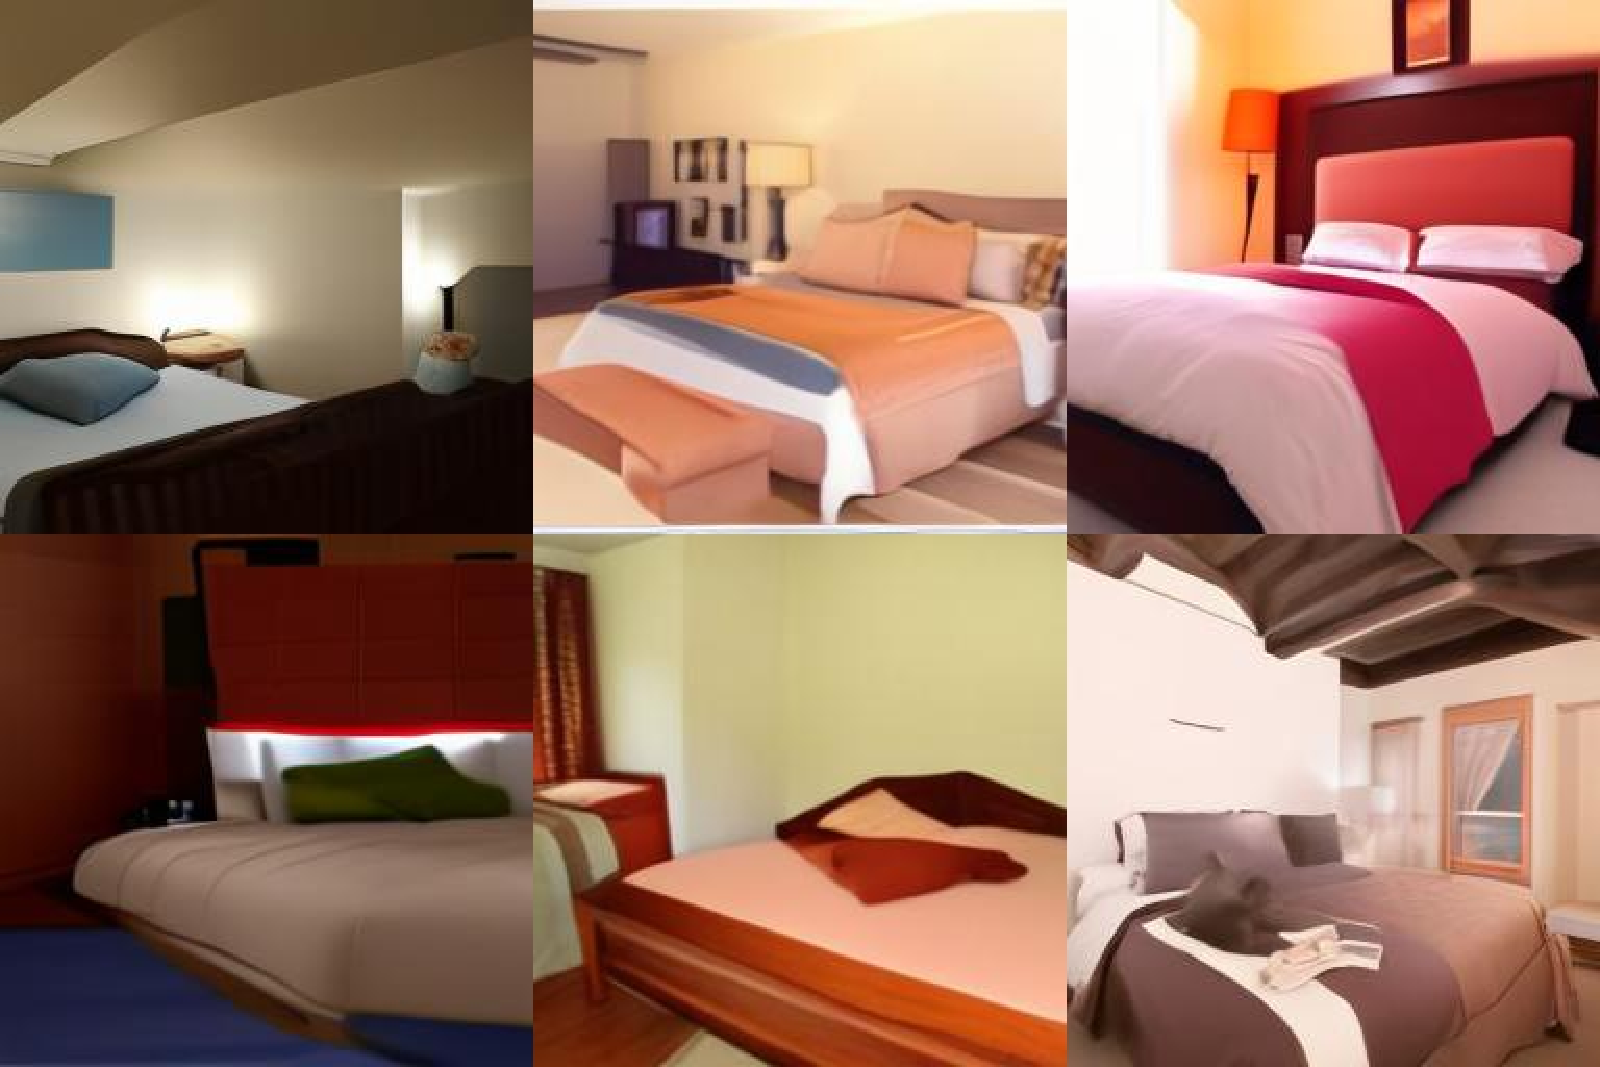
\includegraphics[width=\textwidth]{figures/bedroom/w4a4_e0.pdf}
\caption*{LCQ+MoDiff W4A4}
\label{appfig: bedroom_w4a4}
\end{subfigure}
\hspace{0.5in}
\begin{subfigure}{0.35\linewidth}

\includegraphics[width=\textwidth]{figures/bedroom/w4a4_rt.pdf}
\caption*{LCQ W4A4}
\label{appfig: bedroom_w4a4_rt}
\end{subfigure} 

\caption{Visualization of LSUN-bedrooms $256\times256$ generated using LCQ and LCQ+MoDiff under 4-bit weight quantization precisions.}
\label{appfig:visual_bedroom_w4}
\end{figure*}

\begin{figure*}[ht!]
\center
\begin{subfigure}{0.76\linewidth}

\includegraphics[width=\textwidth]{figures/cifar/w8a32.pdf} 
\caption*{Full Precision (Act) W8A32}
\label{appfig: cifar_w8a32}
\end{subfigure} \\

\begin{subfigure}{0.17\linewidth}

\includegraphics[width=1\textwidth]{figures/cifar/LCQ/w8a8.pdf}
\caption*{LCQ+MoDiff W8A8}
\label{appfig: cifar_w8a8}
\end{subfigure}
\hspace{0.1in}
\begin{subfigure}{0.17\linewidth}

\includegraphics[width=\textwidth]{figures/cifar/LCQ/w8a8_rt.pdf}
\caption*{LCQ W8A8}
\label{appfig: cifar_w8a8_rt}
\end{subfigure}
\hspace{0.1in}
\begin{subfigure}{0.17\linewidth}

\includegraphics[width=\textwidth]{figures/cifar/qdiff/w8a8.pdf}
\caption*{Q-Diff+MoDiff W8A8}
\label{appfig: cifar_w8a8_q}
\end{subfigure}
\hspace{0.1in}
\begin{subfigure}{0.17\linewidth}
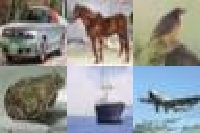
\includegraphics[width=\textwidth]{figures/cifar/qdiff/w8a8_base.pdf}
\caption*{Q-Diff W8A8}
\label{appfig: cifar_w8a8_qb}
\end{subfigure}\\

\begin{subfigure}{0.17\linewidth}

\includegraphics[width=\textwidth]{figures/cifar/LCQ/w8a6.pdf}
\caption*{LCQ+MoDiff W8A6}
\label{appfig: cifar_w8a6}
\end{subfigure}
\hspace{0.1in}
\begin{subfigure}{0.17\linewidth}

\includegraphics[width=\textwidth]{figures/cifar/LCQ/w8a6_rt.pdf}
\caption*{LCQ W8A6}
\label{appfig: cifar_w8a6_rt}
\end{subfigure}
\hspace{0.1in}
\begin{subfigure}{0.17\linewidth}

\includegraphics[width=\textwidth]{figures/cifar/qdiff/w8a6.pdf}
\caption*{Q-Diff+MoDiff W8A6}
\label{appfig: cifar_w8a6_q}
\end{subfigure}
\hspace{0.1in}
\begin{subfigure}{0.17\linewidth}
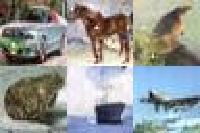
\includegraphics[width=\textwidth]{figures/cifar/qdiff/w8a6_base.pdf}
\caption*{Q-Diff W8A6}
\label{appfig: cifar_w8a6_qb}
\end{subfigure}\\

\begin{subfigure}{0.17\linewidth}

\includegraphics[width=\textwidth]{figures/cifar/LCQ/w8a4.pdf}
\caption*{LCQ+MoDiff W8A4}
\label{appfig: cifar_w8a4}
\end{subfigure}
\hspace{0.1in}
\begin{subfigure}{0.17\linewidth}

\includegraphics[width=\textwidth]{figures/cifar/LCQ/w8a4_rt.pdf}
\caption*{LCQ W8A4}
\label{appfig: cifar_w8a4_rt}
\end{subfigure}
\hspace{0.1in}
\begin{subfigure}{0.17\linewidth}

\includegraphics[width=\textwidth]{figures/cifar/qdiff/w8a4.pdf}
\caption*{Q-Diff+MoDiff W8A4}
\label{appfig: cifar_w8a4_q}
\end{subfigure}
\hspace{0.1in}
\begin{subfigure}{0.17\linewidth}
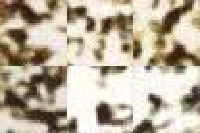
\includegraphics[width=\textwidth]{figures/cifar/qdiff/w8a4_base.pdf}
\caption*{Q-Diff W8A4}
\label{appfig: cifar_w8a4_qb}
\end{subfigure}\\

\begin{subfigure}{0.17\linewidth}

\includegraphics[width=\textwidth]{figures/cifar/LCQ/w8a3.pdf}
\caption*{LCQ+MoDiff W8A3}
\label{appfig: cifar_w8a3}
\end{subfigure}
\hspace{0.1in}
\begin{subfigure}{0.17\linewidth}
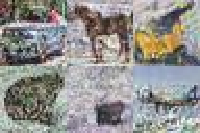
\includegraphics[width=\textwidth]{figures/cifar/LCQ/w8a3_rt.pdf}
\caption*{LCQ W8A3}
\label{appfig: cifar_w8a3_rt}
\end{subfigure}
\hspace{0.1in}
\begin{subfigure}{0.17\linewidth}

\includegraphics[width=\textwidth]{figures/cifar/qdiff/w8a3.pdf}
\caption*{Q-Diff+MoDiff W8A3}
\label{appfig: cifar_w8a3_q}
\end{subfigure}
\hspace{0.1in}
\begin{subfigure}{0.17\linewidth}

\includegraphics[width=\textwidth]{figures/cifar/qdiff/w8a3_base.pdf}
\caption*{Q-Diff W8A3}
\label{appfig: cifar_w8a3_qb}
\end{subfigure}\\

\begin{subfigure}{0.17\linewidth}
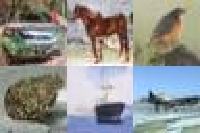
\includegraphics[width=\textwidth]{figures/cifar/LCQ/w8a2.pdf}
\caption*{LCQ+MoDiff W8A2}
\label{appfig: cifar_w8a2}
\end{subfigure}
\hspace{0.1in}
\begin{subfigure}{0.17\linewidth}

\includegraphics[width=\textwidth]{figures/cifar/LCQ/w8a2_rt.pdf}
\caption*{LCQ W8A2}
\label{appfig: cifar_w8a2_rt}
\end{subfigure}
\hspace{0.1in}
\begin{subfigure}{0.17\linewidth}

\includegraphics[width=\textwidth]{figures/cifar/qdiff/w8a2.pdf}
\caption*{Q-Diff+MoDiff W8A2}
\label{appfig: cifar_w8a2_q}
\end{subfigure}
\hspace{0.1in}
\begin{subfigure}{0.17\linewidth}

\includegraphics[width=\textwidth]{figures/cifar/qdiff/w8a2_base.pdf}
\caption*{Q-Diff W8A2}
\label{appfig: cifar_w8a2_qb}
\end{subfigure}
% \caption{}
\caption{Visualization of LSUN-bedrooms $256\times256$ generated using LCQ, LCQ+MoDiff, Q-Diff, and Q-Diff+MoDiff under 8-bit weight quantization precisions.}
\label{appfig:visual_cifar_w8}

\end{figure*}

\begin{figure*}[ht!]
\center
\begin{subfigure}{0.76\linewidth}

\includegraphics[width=\textwidth]{figures/cifar/w4a32.pdf} 
\caption*{Full Precision (Act) w4A32}
\label{appfig: cifar_w4a32}
\end{subfigure} \\

\begin{subfigure}{0.17\linewidth}

\includegraphics[width=\textwidth]{figures/cifar/LCQ/w4a8.pdf}
\caption*{LCQ+MoDiff w4A8}
\label{appfig: cifar_w4a8}
\end{subfigure}
\hspace{0.1in}
\begin{subfigure}{0.17\linewidth}

\includegraphics[width=\textwidth]{figures/cifar/LCQ/w4a8_rt.pdf}
\caption*{LCQ w4A8}
\label{appfig: cifar_w4a8_rt}
\end{subfigure}
\hspace{0.1in}
\begin{subfigure}{0.17\linewidth}

\includegraphics[width=\textwidth]{figures/cifar/qdiff/w4a8.pdf}
\caption*{Q-Diff+MoDiff w4A8}
\label{appfig: cifar_w4a8_q}
\end{subfigure}
\hspace{0.1in}
\begin{subfigure}{0.17\linewidth}
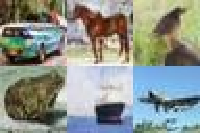
\includegraphics[width=\textwidth]{figures/cifar/qdiff/w4a8_base.pdf}
\caption*{Q-Diff w4A8}
\label{appfig: cifar_w4a8_qb}
\end{subfigure}\\

\begin{subfigure}{0.17\linewidth}

\includegraphics[width=\textwidth]{figures/cifar/LCQ/w4a6.pdf}
\caption*{LCQ+MoDiff w4A6}
\label{appfig: cifar_w4a6}
\end{subfigure}
\hspace{0.1in}
\begin{subfigure}{0.17\linewidth}

\includegraphics[width=\textwidth]{figures/cifar/LCQ/w4a6_rt.pdf}
\caption*{LCQ w4A6}
\label{appfig: cifar_w4a6_rt}
\end{subfigure}
\hspace{0.1in}
\begin{subfigure}{0.17\linewidth}

\includegraphics[width=\textwidth]{figures/cifar/qdiff/w4a6.pdf}
\caption*{Q-Diff+MoDiff w4A6}
\label{appfig: cifar_w4a6_q}
\end{subfigure}
\hspace{0.1in}
\begin{subfigure}{0.17\linewidth}
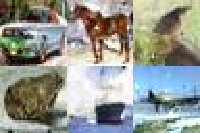
\includegraphics[width=\textwidth]{figures/cifar/qdiff/w4a6_base.pdf}
\caption*{Q-Diff w4A6}
\label{appfig: cifar_w4a6_qb}
\end{subfigure}\\

\begin{subfigure}{0.17\linewidth}

\includegraphics[width=\textwidth]{figures/cifar/LCQ/w4a4.pdf}
\caption*{LCQ+MoDiff w4A4}
\label{appfig: cifar_w4a4}
\end{subfigure}
\hspace{0.1in}
\begin{subfigure}{0.17\linewidth}

\includegraphics[width=\textwidth]{figures/cifar/LCQ/w4a4_rt.pdf}
\caption*{LCQ w4A4}
\label{appfig: cifar_w4a4_rt}
\end{subfigure}
\hspace{0.1in}
\begin{subfigure}{0.17\linewidth}

\includegraphics[width=\textwidth]{figures/cifar/qdiff/w4a4.pdf}
\caption*{Q-Diff+MoDiff w4A4}
\label{appfig: cifar_w4a4_q}
\end{subfigure}
\hspace{0.1in}
\begin{subfigure}{0.17\linewidth}
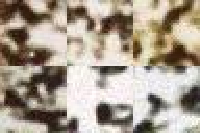
\includegraphics[width=\textwidth]{figures/cifar/qdiff/w4a4_base.pdf}
\caption*{Q-Diff w4A4}
\label{appfig: cifar_w4a4_qb}
\end{subfigure}\\

\begin{subfigure}{0.17\linewidth}

\includegraphics[width=\textwidth]{figures/cifar/LCQ/w4a3.pdf}
\caption*{LCQ+MoDiff w4A3}
\label{appfig: cifar_w4a3}
\end{subfigure}
\hspace{0.1in}
\begin{subfigure}{0.17\linewidth}
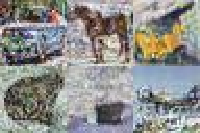
\includegraphics[width=\textwidth]{figures/cifar/LCQ/w4a3_rt.pdf}
\caption*{LCQ w4A3}
\label{appfig: cifar_w4a3_rt}
\end{subfigure}
\hspace{0.1in}
\begin{subfigure}{0.17\linewidth}

\includegraphics[width=\textwidth]{figures/cifar/qdiff/w4a3.pdf}
\caption*{Q-Diff+MoDiff w4A3}
\label{appfig: cifar_w4a3_q}
\end{subfigure}
\hspace{0.1in}
\begin{subfigure}{0.17\linewidth}

\includegraphics[width=\textwidth]{figures/cifar/qdiff/w4a3_base.pdf}
\caption*{Q-Diff w4A3}
\label{appfig: cifar_w4a3_qb}
\end{subfigure}\\

\begin{subfigure}{0.17\linewidth}
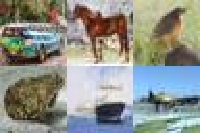
\includegraphics[width=\textwidth]{figures/cifar/LCQ/w4a2.pdf}
\caption*{LCQ+MoDiff w4A2}
\label{appfig: cifar_w4a2}
\end{subfigure}
\hspace{0.1in}
\begin{subfigure}{0.17\linewidth}

\includegraphics[width=\textwidth]{figures/cifar/LCQ/w4a2_rt.pdf}
\caption*{LCQ w4A2}
\label{appfig: cifar_w4a2_rt}
\end{subfigure}
\hspace{0.1in}
\begin{subfigure}{0.17\linewidth}

\includegraphics[width=\textwidth]{figures/cifar/qdiff/w4a2.pdf}
\caption*{Q-Diff+MoDiff w4A2}
\label{appfig: cifar_w4a2_q}
\end{subfigure}
\hspace{0.1in}
\begin{subfigure}{0.17\linewidth}

\includegraphics[width=\textwidth]{figures/cifar/qdiff/w4a2_base.pdf}
\caption*{Q-Diff w4A2}
\label{appfig: cifar_w4a2_qb}
\end{subfigure}
\caption{Visualization of LSUN-bedrooms $256\times256$ generated using LCQ, LCQ+MoDiff, Q-Diff, and Q-Diff+MoDiff under 4-bit weight quantization precisions.}
\label{appfig:visual_cifar_w4}

\end{figure*}
